% Options for packages loaded elsewhere
\PassOptionsToPackage{unicode}{hyperref}
\PassOptionsToPackage{hyphens}{url}
\PassOptionsToPackage{dvipsnames,svgnames,x11names}{xcolor}
%
\documentclass[
  authoryear,
  preprint,
  3p,
  onecolumn]{elsarticle}

\usepackage{amsmath,amssymb}
\usepackage{iftex}
\ifPDFTeX
  \usepackage[T1]{fontenc}
  \usepackage[utf8]{inputenc}
  \usepackage{textcomp} % provide euro and other symbols
\else % if luatex or xetex
  \usepackage{unicode-math}
  \defaultfontfeatures{Scale=MatchLowercase}
  \defaultfontfeatures[\rmfamily]{Ligatures=TeX,Scale=1}
\fi
\usepackage{lmodern}
\ifPDFTeX\else  
    % xetex/luatex font selection
\fi
% Use upquote if available, for straight quotes in verbatim environments
\IfFileExists{upquote.sty}{\usepackage{upquote}}{}
\IfFileExists{microtype.sty}{% use microtype if available
  \usepackage[]{microtype}
  \UseMicrotypeSet[protrusion]{basicmath} % disable protrusion for tt fonts
}{}
\makeatletter
\@ifundefined{KOMAClassName}{% if non-KOMA class
  \IfFileExists{parskip.sty}{%
    \usepackage{parskip}
  }{% else
    \setlength{\parindent}{0pt}
    \setlength{\parskip}{6pt plus 2pt minus 1pt}}
}{% if KOMA class
  \KOMAoptions{parskip=half}}
\makeatother
\usepackage{xcolor}
\setlength{\emergencystretch}{3em} % prevent overfull lines
\setcounter{secnumdepth}{5}
% Make \paragraph and \subparagraph free-standing
\ifx\paragraph\undefined\else
  \let\oldparagraph\paragraph
  \renewcommand{\paragraph}[1]{\oldparagraph{#1}\mbox{}}
\fi
\ifx\subparagraph\undefined\else
  \let\oldsubparagraph\subparagraph
  \renewcommand{\subparagraph}[1]{\oldsubparagraph{#1}\mbox{}}
\fi


\providecommand{\tightlist}{%
  \setlength{\itemsep}{0pt}\setlength{\parskip}{0pt}}\usepackage{longtable,booktabs,array}
\usepackage{calc} % for calculating minipage widths
% Correct order of tables after \paragraph or \subparagraph
\usepackage{etoolbox}
\makeatletter
\patchcmd\longtable{\par}{\if@noskipsec\mbox{}\fi\par}{}{}
\makeatother
% Allow footnotes in longtable head/foot
\IfFileExists{footnotehyper.sty}{\usepackage{footnotehyper}}{\usepackage{footnote}}
\makesavenoteenv{longtable}
\usepackage{graphicx}
\makeatletter
\def\maxwidth{\ifdim\Gin@nat@width>\linewidth\linewidth\else\Gin@nat@width\fi}
\def\maxheight{\ifdim\Gin@nat@height>\textheight\textheight\else\Gin@nat@height\fi}
\makeatother
% Scale images if necessary, so that they will not overflow the page
% margins by default, and it is still possible to overwrite the defaults
% using explicit options in \includegraphics[width, height, ...]{}
\setkeys{Gin}{width=\maxwidth,height=\maxheight,keepaspectratio}
% Set default figure placement to htbp
\makeatletter
\def\fps@figure{htbp}
\makeatother

\usepackage{lineno}\linenumbers \usepackage{multirow} \usepackage{lscape} \newcommand{\blandscape}{\begin{landscape}} \newcommand{\elandscape}{\end{landscape}}
\makeatletter
\makeatother
\makeatletter
\makeatother
\makeatletter
\@ifpackageloaded{caption}{}{\usepackage{caption}}
\AtBeginDocument{%
\ifdefined\contentsname
  \renewcommand*\contentsname{Table of contents}
\else
  \newcommand\contentsname{Table of contents}
\fi
\ifdefined\listfigurename
  \renewcommand*\listfigurename{List of Figures}
\else
  \newcommand\listfigurename{List of Figures}
\fi
\ifdefined\listtablename
  \renewcommand*\listtablename{List of Tables}
\else
  \newcommand\listtablename{List of Tables}
\fi
\ifdefined\figurename
  \renewcommand*\figurename{Figure}
\else
  \newcommand\figurename{Figure}
\fi
\ifdefined\tablename
  \renewcommand*\tablename{Table}
\else
  \newcommand\tablename{Table}
\fi
}
\@ifpackageloaded{float}{}{\usepackage{float}}
\floatstyle{ruled}
\@ifundefined{c@chapter}{\newfloat{codelisting}{h}{lop}}{\newfloat{codelisting}{h}{lop}[chapter]}
\floatname{codelisting}{Listing}
\newcommand*\listoflistings{\listof{codelisting}{List of Listings}}
\makeatother
\makeatletter
\@ifpackageloaded{caption}{}{\usepackage{caption}}
\@ifpackageloaded{subcaption}{}{\usepackage{subcaption}}
\makeatother
\makeatletter
\@ifpackageloaded{tcolorbox}{}{\usepackage[skins,breakable]{tcolorbox}}
\makeatother
\makeatletter
\@ifundefined{shadecolor}{\definecolor{shadecolor}{rgb}{.97, .97, .97}}
\makeatother
\makeatletter
\makeatother
\makeatletter
\makeatother
\journal{Journal Name}
\ifLuaTeX
  \usepackage{selnolig}  % disable illegal ligatures
\fi
\usepackage[]{natbib}
\bibliographystyle{elsarticle-harv}
\IfFileExists{bookmark.sty}{\usepackage{bookmark}}{\usepackage{hyperref}}
\IfFileExists{xurl.sty}{\usepackage{xurl}}{} % add URL line breaks if available
\urlstyle{same} % disable monospaced font for URLs
\hypersetup{
  pdftitle={The effects of drought on land cover change and vegetation productivity in continental Chile},
  pdfauthor={Francisco Zambrano; Anton Vrieling; Francisco Meza; Iongel Duran-Llacer; Francisco Fernández; Alejandro Venegas-González; Nicolas Raab; Dylan Craven},
  pdfkeywords={drought, land cover change, vegetation
productivity, ecosystem},
  colorlinks=true,
  linkcolor={blue},
  filecolor={Maroon},
  citecolor={Blue},
  urlcolor={Blue},
  pdfcreator={LaTeX via pandoc}}

\setlength{\parindent}{6pt}
\begin{document}

\begin{frontmatter}
\title{The effects of drought on land cover change and vegetation
productivity in continental Chile}
\author[1,2]{Francisco Zambrano%
\corref{cor1}%
}
 \ead{francisco.zambrano@umayor.cl} 
\author[3]{Anton Vrieling%
%
}

\author[4,5,6]{Francisco Meza%
%
}

\author[7]{Iongel Duran-Llacer%
%
}

\author[8,9]{Francisco Fernández%
%
}

\author[10]{Alejandro Venegas-González%
%
}

\author[4]{Nicolas Raab%
%
}

\author[12,13]{Dylan Craven%
%
}


\affiliation[1]{organization={Hémera Centro de Observación de la Tierra,
Facultad de Ciencias, Escuela de Ingeniería en Medio Ambiente y
Sustentabilidad, Universidad Mayor},city={Santiago},country={7500994,
Chile.},countrysep={,},postcodesep={}}
\affiliation[2]{organization={Observatorio de Sequía para la Agricultura
y la Biodiversidad de Chile (ODES), Universidad
Mayor},city={Santiago},country={7500994,
Chile.},countrysep={,},postcodesep={}}
\affiliation[3]{organization={Faculty of Geo-Information Science and
Earth, University of Twente},city={Enschede},country={The
Netherlands.},countrysep={,},postcodesep={}}
\affiliation[4]{organization={Facultad de Agronomía y Sistemas
Naturales, Pontificia Universidad Católica de
Chile.},city={Santiago},country={Chile.},countrysep={,},postcodesep={}}
\affiliation[5]{organization={Instituto para el Desarrollo Sustentable.
Pontificia Universidad Católica de
Chile},city={Santiago},country={Chile.},countrysep={,},postcodesep={}}
\affiliation[6]{organization={Centro Interdisciplinario de Cambio
Global, Pontificia Universidad Católica de
Chile},city={Santiago},country={Chile.},countrysep={,},postcodesep={}}
\affiliation[7]{organization={Hémera Centro de Observación de la Tierra,
Facultad de Ciencias, Universidad
Mayor,},city={Santiago},country={7500994,
Chile.},countrysep={,},postcodesep={}}
\affiliation[8]{organization={Center of Economics for Sustainable
Development (CEDES), Faculty of Economics and Government, Universidad
San
Sebastian},city={Santiago},country={Chile.},countrysep={,},postcodesep={}}
\affiliation[9]{organization={Center of Applied Ecology and
Sustainability
(CAPES)},city={Santiago},country={Chile.},countrysep={,},postcodesep={}}
\affiliation[10]{organization={Instituto de Ciencias Agroalimentarias,
Animales y Ambientales (ICA3), Universidad de O'Higgins},city={San
Fernando},country={Chile.},countrysep={,},postcodesep={}}
\affiliation[11]{organization={},,postcodesep={}}
\affiliation[12]{organization={, GEMA Center for Genomics, Ecology \&
Environment, Universidad Mayor, Camino La Pirámide Huechuraba
5750},city={Santiago},country={Chile.},countrysep={,},postcodesep={}}
\affiliation[13]{organization={Data Observatory
Foundation},city={Santiago},country={Chile.},countrysep={,},postcodesep={}}

\cortext[cor1]{Corresponding author}








        
\begin{abstract}
Chile has experienced a persistent decrease in water supply, which
impacts the hydrological system and vegetation development. This
persistent period of water scarcity has been defined as a mega-drought.
There is yet insufficient understanding of ecological drought in Chile
due to the limited studies on the relationship between drought and
ecosystem changes. The aim of our study is to evaluate the interaction
of drought, land cover change, and vegetation productivity over
continental Chile. To assess drought, we used drought indices for
atmospheric evaporative demand (AED), water supply, and soil moisture
from short- (1, 3, 6 months) to long-term (12, 24, 36 months) time
scales. We derived the drought indices using monthly ERA5-Land
reanalysis data from 1981 to 2023. We used Moderate-Resolution Imaging
Spectroradiometer (MODIS) datasets to derive information on annual land
cover and monthly vegetation productivity. Our results showed that,
except for the Austral part, Chile has a temporal decreasing trend in
water supply, and across the whole country, there is an increase in AED.
These trends become stronger over longer time scales. We found a
negative trend in vegetation productivity in the north-central area,
which is more prominent for shrubland and savanna as compared to
croplands and forests. The anomaly in soil moisture over the past 12
months (SSI-12) is the most important variable explaining these changes,
followed by anomalies in accumulated precipitation over one to two years
(SPI-12 and SPI-24). The variable importance obtained by random forest
models indicates that drought explains about 12--41\% of the change in
land cover surface across Chile for forest, grassland, shrubland, and
savanna but has little relation to the changes in croplands. The
increase in AED is the main variable associated with the change in land
cover, followed by a reduction in precipitation and soil moisture. Our
findings provide insightful information that could assist in developing
adaptation measures for Chilean ecosystems to cope with climate change
and drought.
\end{abstract}





\begin{keyword}
    drought \sep land cover change \sep vegetation productivity \sep 
    ecosystem
\end{keyword}
\end{frontmatter}
    \captionsetup{justification=raggedright,singlelinecheck=false}

\ifdefined\Shaded\renewenvironment{Shaded}{\begin{tcolorbox}[breakable, borderline west={3pt}{0pt}{shadecolor}, frame hidden, enhanced, sharp corners, boxrule=0pt, interior hidden]}{\end{tcolorbox}}\fi

\hypertarget{introduction}{%
\section{Introduction}\label{introduction}}

Drought can be classified as 1) meteorological, when precipitation in a
specific period remains below the mean precipitation experienced in the
same period during multiple years (more than 30 years usually); 2)
hydrological, when these anomalies last for long periods (months to
years) and affect water systems; and 3) agricultural, when the deficit
negatively impacts plant health and leads to decreased productivity of
crops or pastures \citep{Wilhite1985}. However, because drought is also
influenced by human activities, \citet{Loon2016} and
\citet{AghaKouchak2021} expanded the drought definition for the
Anthropocene, indicating that the feedback of human decisions and
activities should also be considered (i.e., anthropogenic drought).
Droughts can lead to increased tree mortality \citep{Cheng2024} and
induce alterations in land cover and land use, ultimately affecting
ecosystems \citep{Crausbay2017}. Even though many ecological studies
have at times mistakenly considered ``dry'' conditions as ``drought''
\citep{Slette2019}, ecological drought can be defined as \emph{``an
episodic deficit in water availability that drives ecosystems beyond
thresholds of vulnerability, impacts ecosystem services, and triggers
feedback in natural and/or human systems''} \citep{Crausbay2017}. In
light of current global warming, it is crucial to study the interaction
between drought and ecosystems in order to understand their feedback and
impact on future water security \citep{Bakker2012}.

Global warming, as a result of human-induced greenhouse gas emissions,
has increased the frequency and intensity of drought, according to the
sixth assessment report (AR6) of the Intergovernmental Panel on Climate
Change (IPCC) \citep{IPCC2023}. The evidence supporting this claim has
been strengthened since AR5 \citep{IPCC2013}. Recent studies, however,
have produced contrasting findings, with some suggesting that drought
has not exhibited a significant trend over the past forty years
\citep{Vicente-Serrano2022, Kogan2020}. \citet{Vicente-Serrano2022}
analyzed the trend in meteorological drought on a global scale, finding
that only in a few regions an increase in the severity of drought was
observed. Moreover, they attributed this increase solely to an increase
in atmospheric evaporative demand (AED) due to higher temperatures,
which in turn enhances vegetation water demand, with important
implications for agricultural and ecological droughts. Also, they state
that \emph{``the increase in hydrological droughts has been primarily
observed in regions with high water demand and land cover change, led by
an increase in agricultural land''}. Similarly, \citet{Kogan2020}
analyzed the drought trend using remotely-sensed vegetation health
indicators, finding that for the globe and main grain-producing
countries, drought has not expanded or intensified during the past 38
years. Nonetheless, \citet{IPCC2021} suggests that there is a medium to
high degree of confidence that rising temperatures will increase the
extent, frequency, and severity of agricultural and ecological droughts.
Also, AR6 \citep{IPCC2023} predicts that many regions of the world will
experience more severe agricultural and ecological droughts even if
global warming stabilizes at 1.5°--2°C. To better evaluate the impact of
drought trends on ecosystems, assessments of the relationship between
meteorological and soil moisture variables and their effects on
vegetation are much needed.

From 1960 to 2019, land use change has impacted around one-third of the
Earth's surface, which is four times more than previously thought
\citep{Winkler2021}. Multiple studies aim to analyze and forecast
changes in land cover globally \citep{Winkler2021, Song2018} and
regionally
\citep{Chamling2020, Homer2020, Yang2021, Schulz2010, Echeverria2012}.
Some seek to analyze the impact of land cover change on climate
conditions such as temperature and precipitation
\citep{Luyssaert2014, Pitman2012}. There is less research on drought and
its relation to land cover change and vegetation productivity
\citep{Chen2022, Akinyemi2021, Peng2017}. \citet{Peng2017} utilized net
primary productivity to examine the spatial and temporal variations in
vegetation productivity at global level and assess to what extent
drought influenced this variability by comparing the twelve-month
Standardized Precipitation Evapotranspiration Index (SPEI) and land
cover change. According to their findings, drought is responsible for
37\% of the decline and accounts for 55\% of the variability in
vegetation productivity. \citet{Chen2022} instead found poor
correlations (r\textless0.2) between the vegetation productivity trends
against meteorological drought (SPEI of twelve months in December) and
soil moisture at the global level. These studies mostly looked at how
changes in land cover and vegetation productivity are related to a
single drought index (SPEI) obtained for 12 month periods. SPEI takes
into account the combined effect of precipitation and AED as a water
balance, but it does not allow to know the contribution of each variable
on its own. To better understand these contributions on land cover
change and vegetation productivity the following questions may be asked:
i) how do land cover and vegetation productivity respond to short- to
long-term meteorological and soil moisture droughts? And ii) how is this
response different between humid and arid climatic zones? Likewise,
there is a lack of understanding of how the alteration in water supply
and demand is affecting land cover transformations.

To address the previous questions over extensive regions, we can utilize
gridded data on water availability, vegetation conditions, and the
respective drought indices. For monitoring drought, the World
Meteorological Organization recommends the SPI (Standardized
Precipitation Index) \citep{WMO2012}. The SPI is a multi-scalar drought
index that only uses precipitation to assess short- to long-term
droughts. \citet{Vicente-Serrano2010} proposed the Standardized
Precipitation Evapotranspiration Index (SPEI), which incorporates the
temperature effect by subtracting AED from precipitation. SPEI allows
for analyzing the combined effect of precipitation and AED. Since its
formulation, it has been used worldwide for the study and monitoring of
drought \citep{Gebrechorkos2023, Liu2024}. Recently, there has been more
interest in using AED to track droughts separately to better disentangle
precipitation from temperature-dependent effects
\citep{Vicente-Serrano2020}. One of the reasons is that AED is more
linked to flash droughts in water-limited regions \citep{Noguera2022}.
\citet{Hobbins2016} and \citet{McEvoy2016} developed the Evaporative
Demand Drought Index (EDDI) to monitor droughts solely using the AED,
and it has proven effective in monitoring flash droughts
\citep{Li2024, Ford2023}. For soil moisture, several drought indices
exist, such as the Soil Moisture Deficit Index (SDMI)
\citep{Narasimhan2005} and the Soil Moisture Agricultural Drought Index
(SMADI) \citep{Souza2021}. \citet{Hao2013} and \citet{AghaKouchak2014}
proposed the Standardized Soil Moisture Index (SSI), which has a similar
formulation as the SPI, SPEI, and EDDI. Thus, many drought indices exist
that allow for a comprehensive assessment of drought on short- to
long-term scales and that allow for the use of single variables from
Earth's water balance (e.g., precipitation, AED, soil moisture).
Climatic variability impacts vegetation development, with unfavorable
conditions such as low precipitation and high temperatures usually
promoting a decrease in plant productivity. To monitor the response of
vegetation for large areas, the common practice is to use satellite
data. For example, the Normalized Difference Vegetation Index (NDVI)
derived from frequent satellite observations of red and near infrared
spectral reflectance, has been widely used as a proxy for biomass
production
\citet{Camps-Valls2021};\citet{Paruelo2016};\citet{Helman2014}{]}. For
Chile's cultivated land, \citet{Zambrano2018} used the zcNDVI for
assessing seasonal biomass production in response to drought. Comparing
the various meteo-related and vegetation-based drought indices, we can
further our understanding of the impact of drought on ecosystems.

Chile's diverse climatic and ecosystem types
\citep{Beck2023, Luebert2022} make it an ideal natural laboratory for
studying climate and ecosystems. Additionally, the country has
experienced severe drought conditions that have had significant effects
on vegetation and water storage. North-central Chile has faced a
persistent precipitation deficit since 2010, defined as a mega-drought
\citep{Garreaud2017}, which has impacted the Chilean ecosystem and
consequently makes it highly vulnerable to climate change
\citep{Barria2021, AlvarezGarreton2021}. This mega-drought was defined
by the annual time series of the Standardized Precipitation Index (SPI)
at a time scale of twelve months at the end of each year (December) when
having values below one standard deviation. Some studies have addressed
how this drought affects single ecosystems in terms of forest growth
\citep{Miranda2020, Venegas2018}, forest fire occurrence
\citep{UrrutiaJalabert2018}, and crop productivity
\citep[\citet{Zambrano2016}]{Zambrano2023, Zambrano2018}. The term
``mega-drought'' is used in Chile to describe a prolonged water shortage
that lasts for several years, resulting in a permanent deficit that
impacts the hydrological system \citep{Boisier2018}. Therefore, it is
crucial to evaluate temporal scales that consider the cumulative impact
over a period of several years. In Chile, the relationship between
drought and the environment remains poorly understood. Hence, we aim to
contribute to understanding how climatic and soil moisture droughts
influence ecosystem dynamics in order to provide useful information that
helps for a better understanding of ecological droughts and, at the same
time, helps to make well-informed decisions on adaptation strategies.

Here, we analyze the multi-dimensional impacts of drought across
ecosystems in continental Chile. More specifically, we aim to assess: i)
short- to long-term temporal trends in multi-scalar drought indices; ii)
temporal changes in land-use cover and the direction and magnitude of
their relationships with trends in drought indices; and iii) the trend
in vegetation productivity and its relationship with drought indices
across Chilean ecosystems.

\hypertarget{study-area}{%
\section{Study area}\label{study-area}}

Continental Chile has diverse climate conditions with strong gradients
from north to south and east to west \citep{Aceituno2021}
Figure~\ref{fig-studyArea}a, which determines its great ecosystem
diversity \citep{Luebert2022} (Figure~\ref{fig-studyArea}c). The Andes
Mountains are a main factor in climate variation \citep{Garreaud2009}.
For an aggregated overview of the results of the study, we used the five
Chilean macrozones: ``Norte Grande'' (17°34'--25°42'S), ``Norte Chico''
(25°42'-32°8'S), ``Centro'' (32°08'-36°12'S), ``Sur'' (36°12'-43°48'S),
and ``Austral'' (43°48'-56°00'S). ``Norte Grande'' and ``Norte Chico''
predominate in an arid desert climate with hot (Bwh) and cold (Bwk)
temperatures. At the south of ``Norte Chico'', the climate changes to an
arid steppe with cold temperatures (Bsk). In these two northern regions,
the land is mostly bare, with a small surface of vegetation types such
as shrubland and grassland. In the macrozones ``Centro'' and the
northern half of ``Sur'', the main climate is Mediterranean, with warm
to hot summers (Csa and Csb). Land cover in ``Centro'' comprises a
significant amount of shrubland and savanna (50\%), grassland (16\%),
forest (8\%), and croplands (5\%). An oceanic climate (Cfb) predominates
in the south of ``Sur'' and the north of ``Austral''. Those zones have a
large area of forest and grassland. The southern part of the country has
a tundra climate, while ``Austral'' is a cold semi-arid area with an
extended surface of grassland, forest, and, to a lesser extent, savanna.

\begin{figure*}[!ht]

{\centering 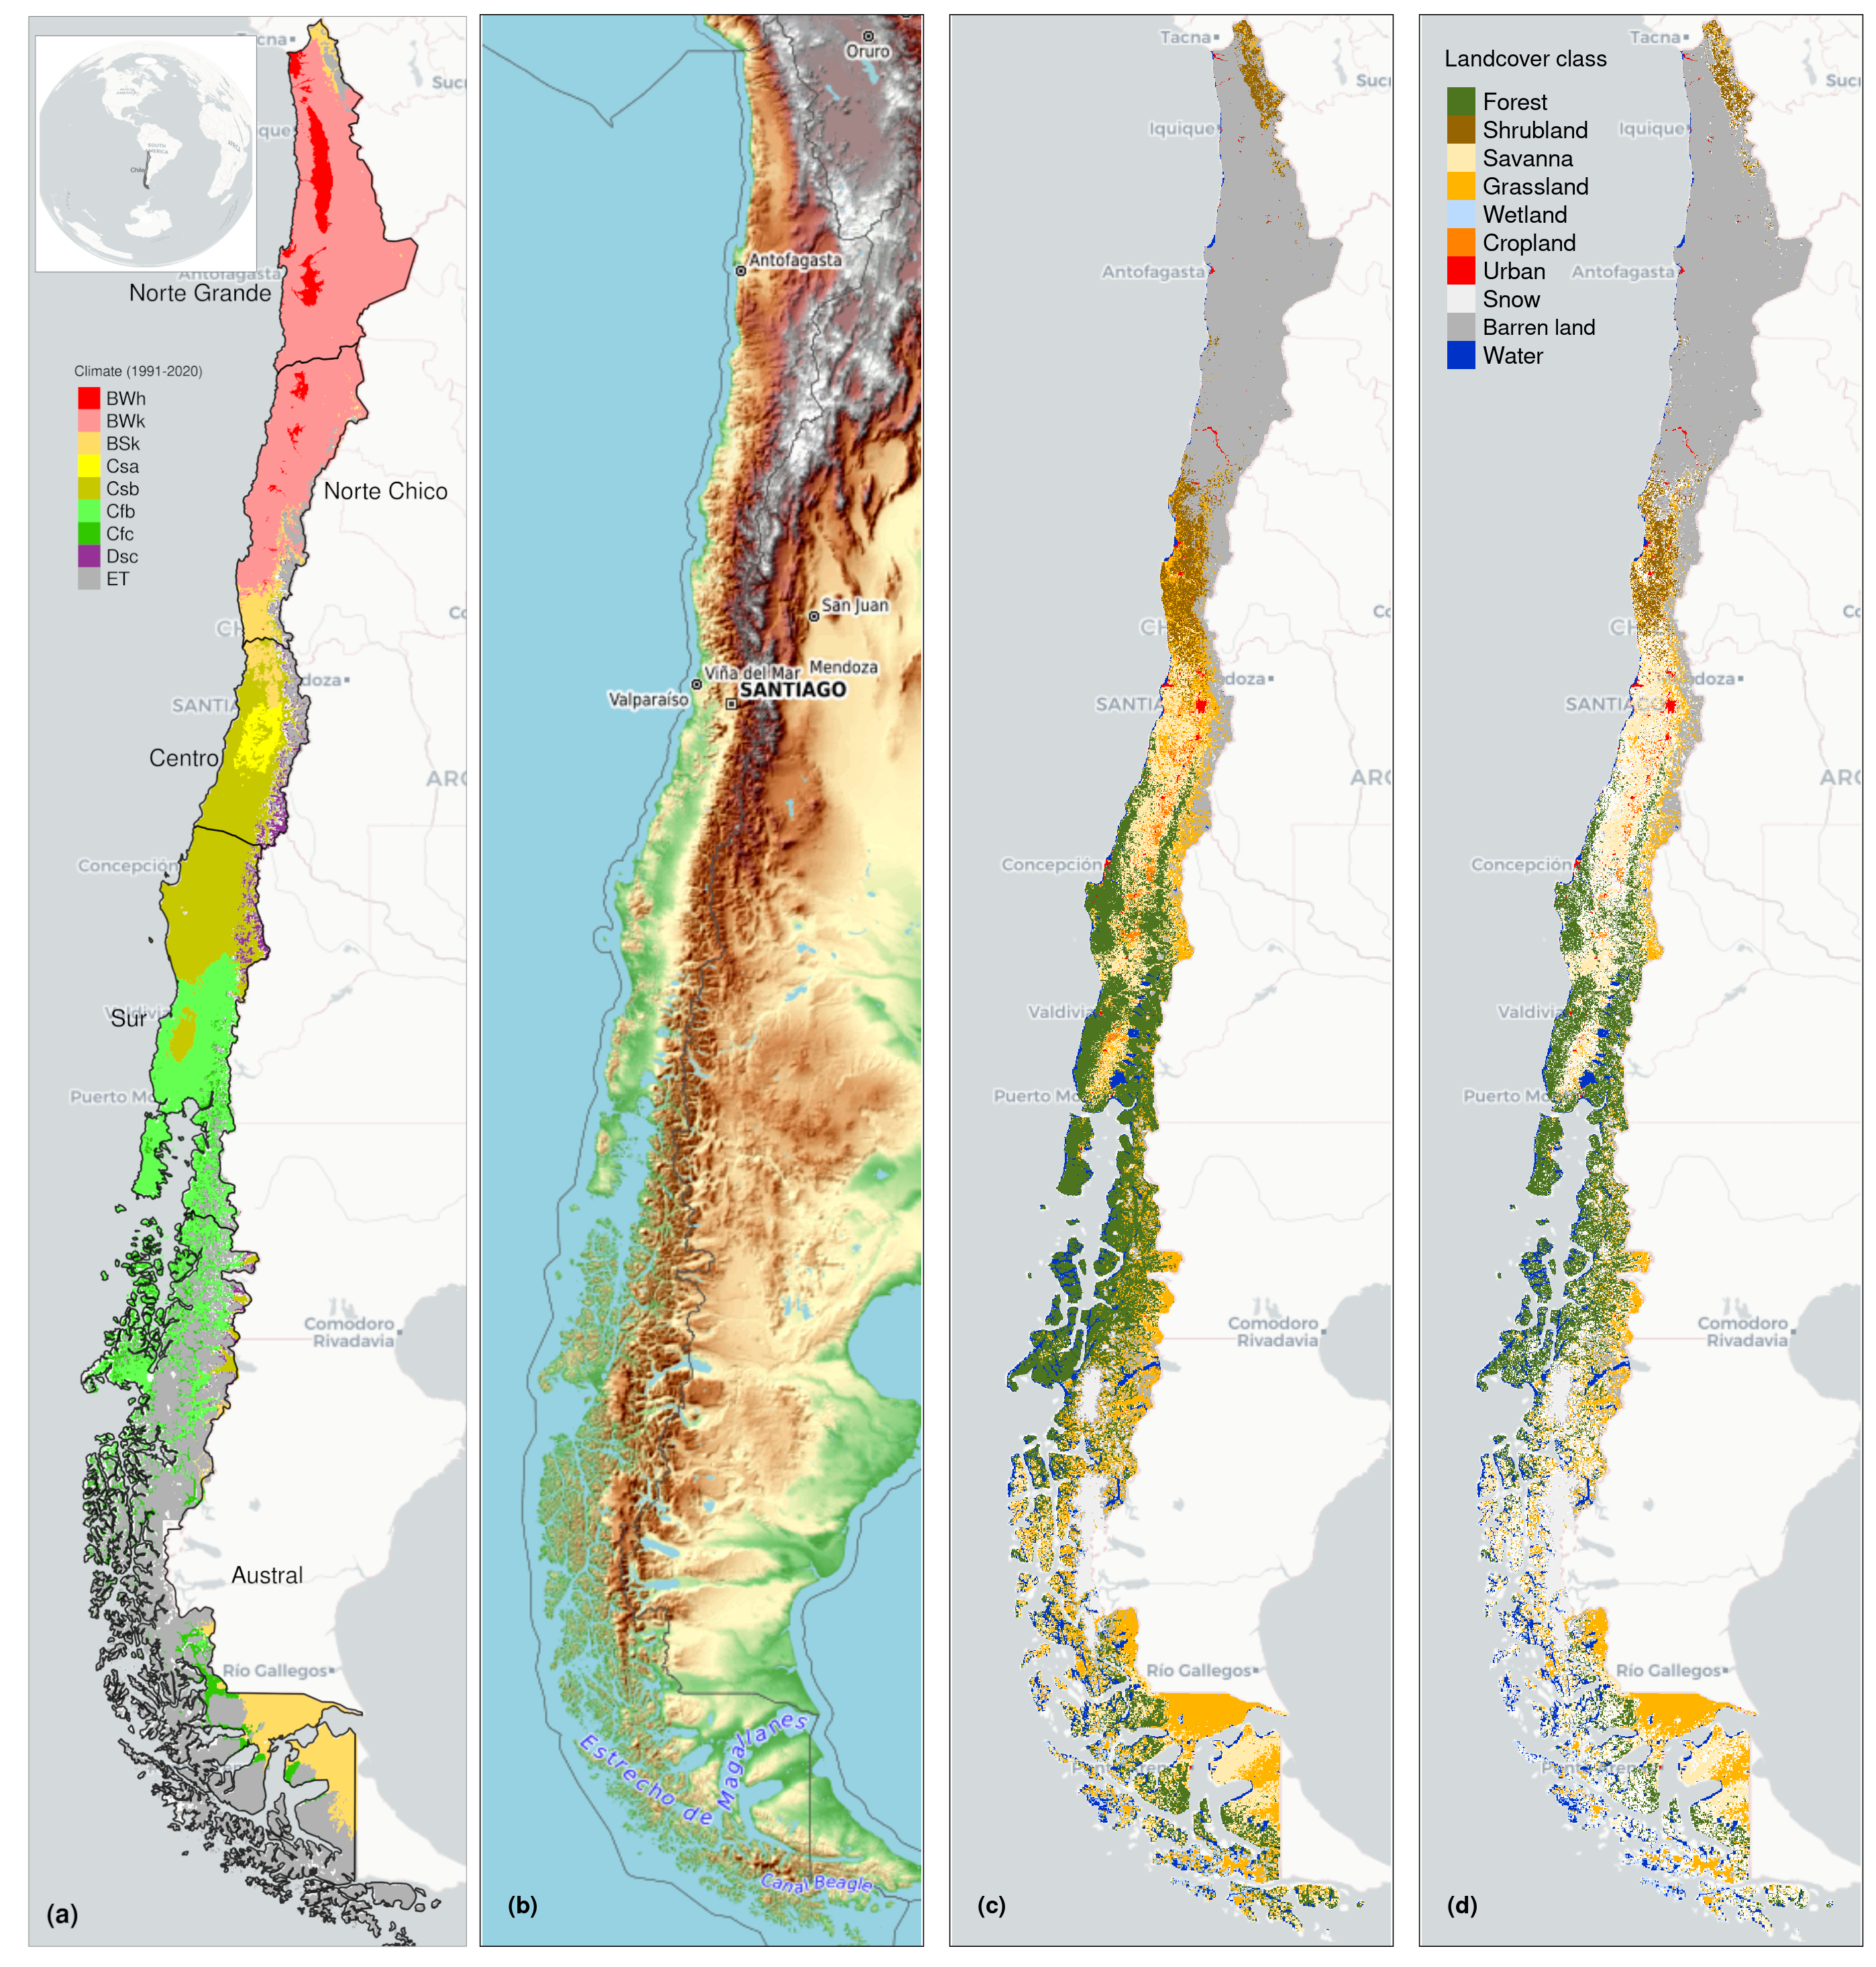
\includegraphics{../output/figs/map_study_con_landcover.png}

}

\caption{\label{fig-studyArea}(a) Chile with the Koppen-Geiger climate
classes and the five macrozones ``Norte Grande'', ``Norte Chico'',
``Centro'', ``Sur'', and ``Austral''. (b) Topography reference map. (c)
land cover classes for 2022. (d) Persistent land cover classes
(\textgreater{} 80\%) for 2001-2022}

\end{figure*}

\hypertarget{materials-and-methods}{%
\section{Materials and Methods}\label{materials-and-methods}}

\hypertarget{data}{%
\subsection{Data}\label{data}}

\hypertarget{gridded-meteorological-and-vegetation-data}{%
\subsubsection{Gridded meteorological and vegetation
data}\label{gridded-meteorological-and-vegetation-data}}

To analyze land cover change, we used the classification scheme by the
IGBP (International Geosphere-Biosphere Programme) from the product
MCD12Q1 Collection 6.1 from MODIS. The MCD12Q1 product is produced for
each year from 2001 to 2022 and defines 17 classes (see Table S1). To
maintain our focus on a large scale and follow the FAO classification
\citep{FAO2022}, we considered native and planted forests as
``forests'', which represent ecosystems dominated by larger trees. To
derive a proxy for vegetation productivity, we used the Normalized
Difference Vegetation Index (NDVI) from the product MOD13A3 Collection
6.1 from MODIS \citep{Didan2015}. MOD13A3 provides vegetation indices
with 1km spatial resolution and monthly frequency. The NASA EOSDIS Land
Processes Distributed Active Archive Center (LP DAAC), USGS Earth
Resources Observation and Science (EROS) Center, Sioux Falls, South
Dakota, provided the MOD13A3 and MCD12Q1 from the online Data Pool,
accessible at \url{https://lpdaa.usgs.gov/tools/data-pool/}.

\begin{table}[!ht]
\caption{Description of the satellite and reanalysis data used}
\label{tab-desEOD}
\scriptsize
\centering
\begin{tabular}{p{0.1\textwidth}cp{0.3\textwidth}p{0.095\textwidth}ccc}
\hline
\multirow{1}{*}{\centering Product} & Sub-product & Variable & Spatial Resolution  & Period & Units & Short Name \\ 
\hline
\multirow{4}{*}{ERA5L} & ~ & Precipitation & \multirow{4}{*}{~0.1°} & \multirow{4}{*}{1981-2023} & mm & P \\ 
         &  & Maximum temperature & ~ & & $°C$ & $T_{max}$ \\ 
         &  & Minimum temperature & ~ & & $°C$ & $T_{min}$ \\ 
         &  & Volumetric Soil Water Content at 1m & ~ & & $m3/m3$ & SM \\ 
ERA5L* & & Atmospheric Evaporative Demand & 0.1° & 1981-2023 & mm & AED \\
        \multirow{2}{*}{MODIS} & MOD13A3.061 & Normalized Difference Vegetation Index & \multirow{2}{*}{~1 km} & 2000-2023 & ~ & NDVI \\ 
         & MCD12Q1.061 & land cover IGBP scheme & & 2001-2022 & ~ & land cover \\ 
\hline
\end{tabular}
{\raggedright *Calculated from maximum and minimum temperatures derived from ERA5L with Eq. \ref{eq-AED}. \par}
\end{table}

For soil moisture, water supply, and water demand variables, we used
ERA5-Land (ERA5L) (ECMWF Reanalysis version 5 over land)
\citep{MunozSabater2021}, a reanalysis dataset that provides the
evolution of atmospheric and land variables since 1950. It has a spatial
resolution of 0.1° (9 km), hourly frequency, and global coverage. We
selected the variables for total precipitation, maximum and minimum
temperature at 2 meters, and volumetric soil water layers between 0 and
100 cm of depth (layer 1 to layer 3). Table \ref{tab-desEOD} shows a
summary of the data and its main characteristics.

\hypertarget{short--to-long-term-drought-trends}{%
\subsection{Short- to long-term drought
trends}\label{short--to-long-term-drought-trends}}

\hypertarget{atmospheric-evaporative-demand-aed}{%
\subsubsection{Atmospheric Evaporative Demand
(AED)}\label{atmospheric-evaporative-demand-aed}}

To compute the drought indices that use water demand, it is necessary to
first calculate the AED. To do this, we employed the Hargreaves method
\citep{Hargreaves1994, Hargreaves1985} by applying the following
equation:

\begin{equation}\protect\hypertarget{eq-AED}{}{AED = 0.0023\cdot Ra\cdot (T+17.8)\cdot (T_{max}-T_{min})^{0.5}}\label{eq-AED}\end{equation}

where \(Ra\) \((MJ\,m^2\, day^{-1})\) is extraterrestrial radiation;
\(T\), \(T_{max}\), and \(T_{min}\) are mean, maximum, and minimum
temperature \((°C)\) at 2m. For calculating \(Ra\) we used the
coordinate of the latitud of the centroid of each pixel as follow:

\begin{equation}\protect\hypertarget{eq-Ra}{}{R_a = \frac{14,400}{\pi}\cdot G_{sc}\cdot d_r \left[\omega_s\cdot sin(\phi)\cdot sin(\delta)+cos(\phi)\cdot cos(\delta)\cdot sin(\omega_s) \right]}\label{eq-Ra}\end{equation}

where:

\(Ra\): extraterrestrial radiation \([MJ\, m^{-2} day-1]\),\\
\(G_{sc}\): solar constant = 0.0820 \([MJ\,m^{-2} min^{-1}]\),\\
\(d_r\): inverse relative distance Earth-Sun,\\
\(\omega_s\) sunset hour angle \([rad]\),\\
\(\phi\): latitude \([rad]\),\\
\(\delta\): solar declination \([rad]\).

We chose the method of Hargreaves to estimate AED because of its
simplicity, which only requires temperatures and extrarrestrial
radiation. Also, it has been recommended over other methods (e.g.,
Penman-Monteith) when the access to climatic variables is limited
\citep{Vicente-Serrano2014}.

\hypertarget{non-parametric-calculation-of-drought-indices}{%
\subsubsection{Non-parametric calculation of drought
indices}\label{non-parametric-calculation-of-drought-indices}}

To derive the drought indices of water supply and demand, soil moisture,
and vegetation (i.e., the proxy of productivity), we used the ERA5L
dataset and the MODIS product, with a monthly frequency for 1981--2023
and 2000--2023, respectively. The drought indices correspond to a
historical anomaly of a variable (e.g., meteorological, vegetation, or
soil moisture). To account for the anomaly, the common practice is to
derive it following a statistical parametric method in which it is
assumed that the statistical distribution of the data is known
\citep{Heim2002}. The use of an erroneous statistical distribution that
does not fit the data is usually the highest source of uncertainty
\citep{Laimighofer2022}. In the case of Chile, due to its high degree of
climatic variability, it is difficult to choose a proper distribution
without previous research that could be applicable throughout Chile.
Here, we follow a non-parametric method for the calculation of the
drought indices, in a similar manner as the framework proposed by
\citet{Farahmand2015}.

For the purpose of monitoring water supply drought, we used the
well-known Standardized Precipitation Index (SPI), which relies on
precipitation data. To evaluate water demand, we chose the Evaporative
Demand Drought Index (EDDI), developed by \citet{Hobbins2016} and
\citet{McEvoy2016}, which is based on the AED. The United States
currently monitors drought using the EDDI (https://psl.noaa.gov/eddi/)
as an experimental index. To consider the combined effect of water
supply and demand, we selected the SPEI \citep{Vicente-Serrano2010}. For
SPEI, an auxiliary variable \(D=P-AED\) is calculated. Soil moisture is
the main driver of vegetation productivity, particularly in semi-arid
regions \citep{Li2022}. Hence, for soil water drought, we used the SSI
(Standardized Soil Moisture Index) \citep{Hao2013}. For the SSI, we used
the average soil moisture from ERA5L at 1m depth. Finally, for the proxy
of productivity, we used the zcNDVI \citep{Zambrano2018}, which was
derived from the monthly time series of NDVI derived from MOD13A1. All
the indices are multi-scalar and can be used for the analysis of short-
to long-term droughts.

To derive the drought indices, we first calculate the sum of the
variables with regard to the time scale(s). In this case, for
generalization purposes, we will use \(V\), referring to variables
\(P\), \(AED\), \(D\), \(NDVI\), and \(SM\) (Table \ref{tab-desEOD}). We
accumulated each over the time series of values (months), and for the
time scales \(s\):

\begin{equation}\protect\hypertarget{eq-sumvar}{}{A^s_i = \sum_{i=n-s-i+2}^{n-i+1} V_i\,\, \forall\, i\geq n-s+1  }\label{eq-sumvar}\end{equation}

The \(A^s_i\) corresponds to a moving window (convolution) that sums the
variable for time scales \(s\). This summation is done over \(s\)
months, starting from the most recent month (\(n\)) back in time until
month \(n-s+1\). For example, using as a variable the precipitation, a
period of twelve months (\(n\)), and a time scale of three months
(\(s\)), it will be:

\[
\begin{split}
A^3_1 &= P_{oct} +P_{nov} +P_{dic} \\
\vdots\,\,\, &= \,\,\,\vdots + \,\,\,\vdots + \,\,\,\vdots \\
A^3_{10} &= P_{jan}+P_{feb} +P_{mar}
\end{split}
\]

Then, we used the empirical Tukey plotting position \citep{Wilks2011}
over \(A_i^s\) to derive the \(P(A_i^s)\) probabilities across a period
of interest:

\begin{equation}\protect\hypertarget{eq-probPai}{}{P(A^s_i) = \frac{i-0.33}{n+0.33'}}\label{eq-probPai}\end{equation}

An inverse normal approximation \citep{Abramowitz1968} obtains the
empirically derived probabilities once the variable cumulates over time
for the scale \(s\). Thus, the drought indices \(SPI\), \(SPEI\),
\(EDDI\), \(SSI\), and \(zcNDVI\) and obtained following the equation:

\begin{equation}\protect\hypertarget{eq-DI}{}{DI(A^s_i) = W - \frac{C_0+C_1\cdot W + c_2 \cdot W^2}{1+d_1\cdot W +d_2\cdot W^2 +d_3\cdot W^3}}\label{eq-DI}\end{equation}

\(DI\) is referring to the drought index calculated for the variable
\(V\) (i.e., SPI, SPEI, EDDI, SSI, and zcNDVI). The values for the
constats are: \(C_0 = 2.515517\), \(C_1 = 0.802853\),
\(C_2 = 0.010328\), \(d_1 = 1.432788\), \(d_2 = 0.189269\), and
\(d3 = 0.001308\). For \(P(A^s_i) \leq 0.5\),
W=\(\sqrt{-2\cdot ln(P(A^s_i))}\) , and for \(P(A^s_i) > 0.5\), replace
\(P(A^s_i)\) with \(1-P(A^s_i)\) and reverse the sign of \(DI(A^s_i)\).

The drought indices were calculated for time scales of 1, 3, 6, 12, 24,
and 36 months at a monthly frequency for 1981--2023 in order to be used
for short- to long-term evaluation of drought.

For the proxy of vegetation productivity, we chose the time scale that
best correlates with annual net primary productivity (NPP) across
continental Chile. For this purpose, we calculated the zcNDVI for time
scales of 1, 3, 6, and 12 months in December and compared it with the
annual NPP. We used the NPP from the MOD17A3HGF \citep{Running2019}
dataset (MODIS). We chose to use six months because the \(R^2\) between
zcNDVI and NPP reaches its highest value at six months. We obtained an
\(R^2\) of 0.31 for forest and 0.72 for shrubland (refer to the
supplementary material in Section S5). Then, we chose the proxy of
vegetation productivity for six months, which we will name zcNDVI
hereafter. It was calculated at a monthly frequency for 2000--2023.

\hypertarget{trend-of-drought-indices}{%
\subsubsection{Trend of drought
indices}\label{trend-of-drought-indices}}

To estimate if there are significant positive or negative trends for the
drought indices, we used the non-parametric Mann-Kendall test
\citep{Kendall1975}. To determine the magnitude of the trend, we used
Sen's slope \citep{Sen1968}. Sen's slope has the advantage over normal
regression that it is less affected by outliers, and as a non-parametric
method it is not influenced by the distribution of the data. We applied
the Mann-Kendall test to see if the trend was significant and Sen's
slope to estimate the magnitude of the trend. We did this for the
indices SPI, EDDI, SPEI, and SSI using the six time scales with data
from 1981 to 2023 (monthly frequency), resulting in 24 trends (per index
and time scale). Then, we extracted the trend aggregated by each of the
five macrozones: ``Norte Grande'' to ``Austral'', and per land cover
type: grassland, forest, cropland, shrubland, savanna, and barren land
(Figure~\ref{fig-studyArea}d).

\hypertarget{interaction-of-land-cover-and-drought}{%
\subsection{Interaction of land cover and
drought}\label{interaction-of-land-cover-and-drought}}

\hypertarget{land-cover-change}{%
\subsubsection{Land cover change}\label{land-cover-change}}

To analyze the land cover change, we use the IGBP scheme from the
MCD12Q1 Collection 6.1 from MODIS. This product has been previously used
for studies of drought and land cover in Chile
\citep{Fuentes2021, Zambrano2018}. We regrouped the 17 classes into ten
macroclasses, as follows: classes 1-4 to forest, 5-7 to shrublands, 8-9
to savannas, 10 as grasslands, 11 as wetlands, 12 and 14 to croplands,
13 as urban, 15 as snow and ice, 16 as barren, and 17 to water bodies
(Table S1). Thus, we have a land cover raster time series with the ten
macroclasses for 2001 and 2023. We validate the land cover macroclasses
regarding a highly detailed (30 m of spatial resolution) land cover map
made for Chile by \citet{Zhao2016} for 2013-2014. Our results showed a
global accuracy of \textasciitilde0.82 and a F1 score of
\textasciitilde0.66. Section S2 in the Supplementary Material shows the
procedure for validation.

We calculated the surface occupied per land cover class into the five
macrozones (``Norte Grande'' to ``Austral'') per year for 2001--2022.
After that, we calculated the trend's change in surface per land cover
type and macroclass. We used Mann-Kendall for the significance of the
trend \citep{Kendall1975} and Sen's slope to calculate the magnitude
\citep{Sen1968}.

To assess how water demand and supply, and soil moisture affect the
variation in vegetation productivity across various land cover types, we
avoid analyzing areas that experienced major land cover changes in the
2021--2022 period. To assess how zcNDVI varied irrespective of land
cover change, we developed a persistence mask for land cover, which only
retains pixels for which the macroclass remained the same for at least
80\% of the 22 years (Figure~\ref{fig-studyArea}d).

\hypertarget{relationship-between-land-cover-and-drought-trends}{%
\subsubsection{Relationship between land cover and drought
trends}\label{relationship-between-land-cover-and-drought-trends}}

To identify which drought indices and time scales have a major impact on
changes in land cover type, we examined the relationship between the
trend in land cover classes and the trend in drought indices. To have
more representative results, we conducted the analysis over sub-basins
within continental Chile. We used 469 basins, which have a surface area
between 0.0746 and 24,000 \(km^2\) and a median area of 1,249 \(km^2\).
For each basin, we calculated the trend per land cover type, considering
the proportion of the type relative to the total surface of the basin.
Then, we extracted per basin the average trend (Sen's slope) of the
drought indices SPI, SPEI, EDDI, SSI, and all their time scales 1, 3, 6,
12, 24, and 36. Also, we extracted the average trend in the proxy of
vegetation productivity (zcNDVI).

We model the trends in land cover per macroclass with the aim of
assessing how land cover trends relate to drought indices. We used the
random forest method \citep{Ho1995}, which employs multiple decision
trees, allowing for classification and regression. Some advantages
include the ability to find non-linear relationships, reduce
overfitting, and derive variable importance. We included the four
drought indices per six time scales and the zcNDVI, totaling 25
predictors. As a result, we created thirty random forest models, one for
each land cover macroclass trend and per macrozone. Each model was
trained using 1000 forests in a resampling scheme to obtain more
reliable results regarding variable importance. We resampled by creating
ten folds, running a random forest per fold, and calculating the
\(R^2\), root mean square error (RMSE), and variable importance. The
variable importance helps for a better understanding of the
relationships by finding which variable has a higher contribution to the
model. Thus, we calculated the variable's importance by permuting
out-of-bag (OOB) data per tree and computing the mean standard error in
the OOB. After permuting each predictor variable, we repeated the
process for the remaining variable. We repeated this process ten times
(per fold) to obtain the performance metrics (\(R^2\), RMSE, and
variable importance).

Finally, we visually explored the connection between the SPI, EDDI, and
SSI drought indices for short- and long-term changes in land cover. To
do this, we compared the relative changes in land cover surface (in
terms of the total surface area per land cover type and macrozone) with
the drought indices of six (short-term) and thirty-six months
(long-term).

\hypertarget{drought-impacts-on-vegetation-productivity}{%
\subsection{Drought impacts on vegetation
productivity}\label{drought-impacts-on-vegetation-productivity}}

For each land cover macroclass, we analyzed the trend of vegetation
productivity over the unchanged land cover macroclasses. To achieve
this, we used the persistent mask of land cover macroclasses, thus
reducing the possibility of evaluating productivity trends that are due
to year-to-year variation in land cover. We used the zcNDVI as a proxy
of vegetation productivity. To assess productivity in Chile's cultivated
land, \citet{Zambrano2018} used the zcNDVI for assessing seasonal
biomass production in relation to climate.

We examined the drought indices of water demand, water supply, and soil
moisture and their correlation with vegetation productivity. The
objective is to determine to what extent soil moisture and water demand
and supply affect vegetation productivity, thus addressing three main
questions: 1) Which of the drought variables---supply, demand, or soil
moisture---helps most in explaining the changes in vegetation
productivity? 2) How do the short- to long-term time scales of the
drought variable affect vegetation productivity in Chile, and how strong
is the relationship? And finally, 3) how does the correlation vary
per-land cover type? Answering these questions should advance our
understanding of how climate is affecting vegetation, considering the
impact on the five land cover types: forest, cropland, grassland,
savanna, and shrubland.

We conducted an analysis on the linear correlation between the indices
SPI, SPEI, EDDI, and SSI over time periods of 1, 3, 6, 12, 24, and 36
months with zcNDVI. We used a method similar to that used by
\citet{Meroni2017} which compared the SPI time-scales with the
cumulative fAPAR (fraction of Absorbed Photosynthetically Active
Radiation). We performed a pixel-to-pixel linear correlation analysis
for each index within the persistent mask of land cover macroclasses. We
first compute the Pearson coefficient of correlation for each of the six
time scales. A time scale is identified as the one that attains the
highest correlation (p \textless{} 0.05). We then extracted the Pearson
correlation coefficient corresponding to the time scales where the value
peaked. As a result, for each index, we generated two raster maps: 1)
containing the raster with values of the time scales and drought index
that reached the maximum correlation, and 2) having the magnitude of the
correlation obtained by the drought index at the time scales.

\hypertarget{software}{%
\subsection{Software}\label{software}}

For the downloading, processing, and analysis of the spatio-temporal
data, we used the open source software for statistical computing and
graphics, R \citep{R2023}. For downloading ERA5L, we used the \{ecmwfr\}
package \citep{Hufkens2019}. For processing raster data, we used
\{terra\} \citep{Hijmans2023} and \{stars\} \citep{Pebesma2023}. For
managing vectorial data, we used \{sf\} \citep{Pebesma2018}. For the
calculation of AED, we used \{SPEI\} \citep{Bergueria2023}. For mapping,
we used \{tmap\} \citep{Tennekes2018}. For data analysis and
visualization, the suite \{tidyverse\} \citep{Wickham2019} was used. For
the random forest modeling, we used the \{tidymodels\} \citep{Kuhn2020}
and \{ranger\} \citep{Wright2017} packages.

\hypertarget{results}{%
\section{Results}\label{results}}

\hypertarget{short--to-long-term-drought-trends-1}{%
\subsection{Short- to long-term drought
trends}\label{short--to-long-term-drought-trends-1}}

Figure~\ref{fig-trendDI} shows the spatial variation of the trend for
the drought indices from short- to long-term scales. SPI and SPEI have a
decreasing trend from ``Norte Chico'' to ``Sur'', but an increasing
trend in ``Austral''. The degree of the trend is larger at higher time
scales. In ``Norte Grande'', the SSI increased in the southwest and
decreased in the northeast, for all time scales. Similar to SPI and
SPEI, SSI decreases at higher time scales. EDDI showed a positive trend
for the whole of continental Chile, with a higher slope toward the north
and a descending gradient toward the south. The slope of trend increases
at higher time scales.

\blandscape

\begin{figure}

\begin{minipage}[t]{0.50\linewidth}

{\centering 

\raisebox{-\height}{

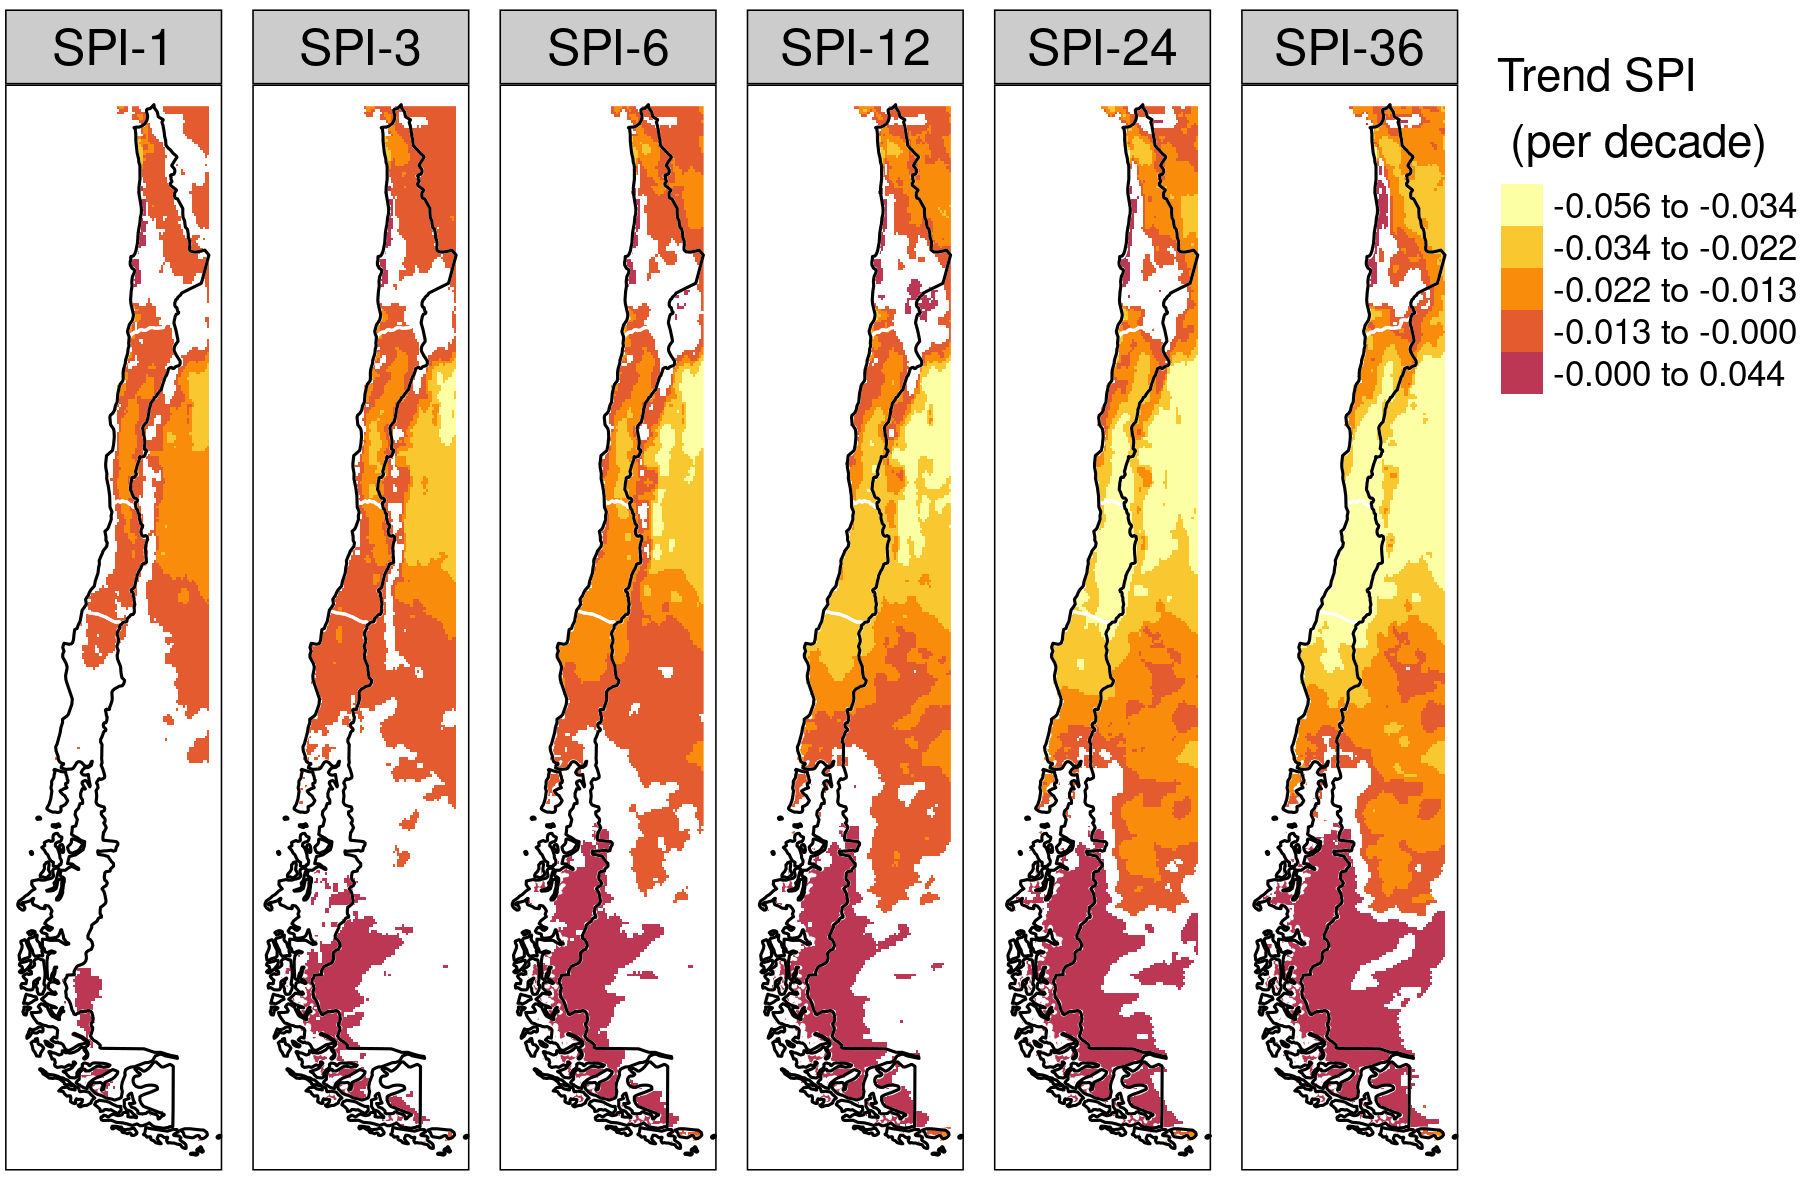
\includegraphics{../output/figs/trend_raster_SPI_1981-2023.png}

}

}

\subcaption{\label{fig-trendDI-1}SPI (Standardized Precipitation Index)}
\end{minipage}%
%
\begin{minipage}[t]{0.50\linewidth}

{\centering 

\raisebox{-\height}{

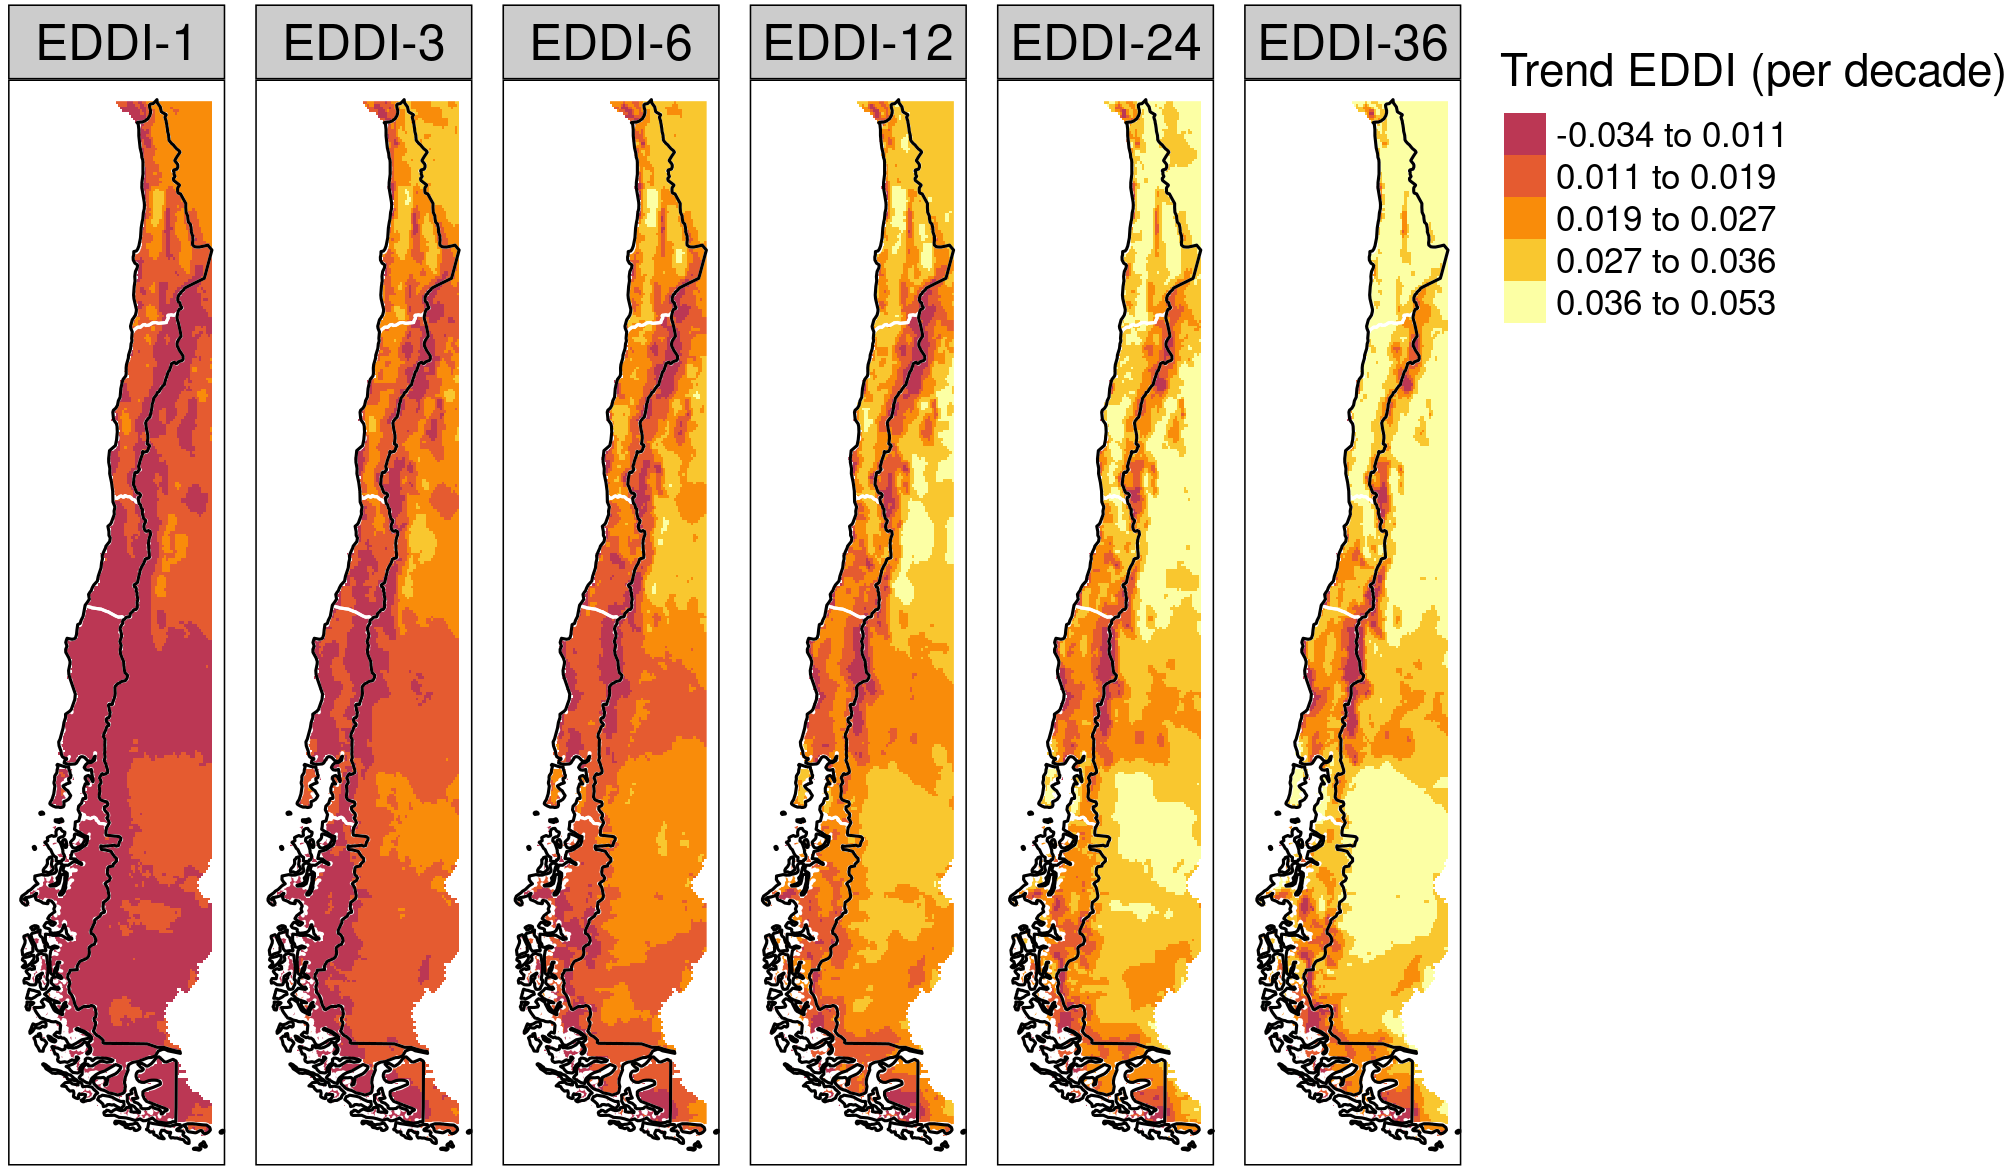
\includegraphics{../output/figs/trend_raster_EDDI_1981-2023.png}

}

}

\subcaption{\label{fig-trendDI-2}EDDI (Evaporative Demand Drought
Index)}
\end{minipage}%
\newline
\begin{minipage}[t]{0.50\linewidth}

{\centering 

\raisebox{-\height}{

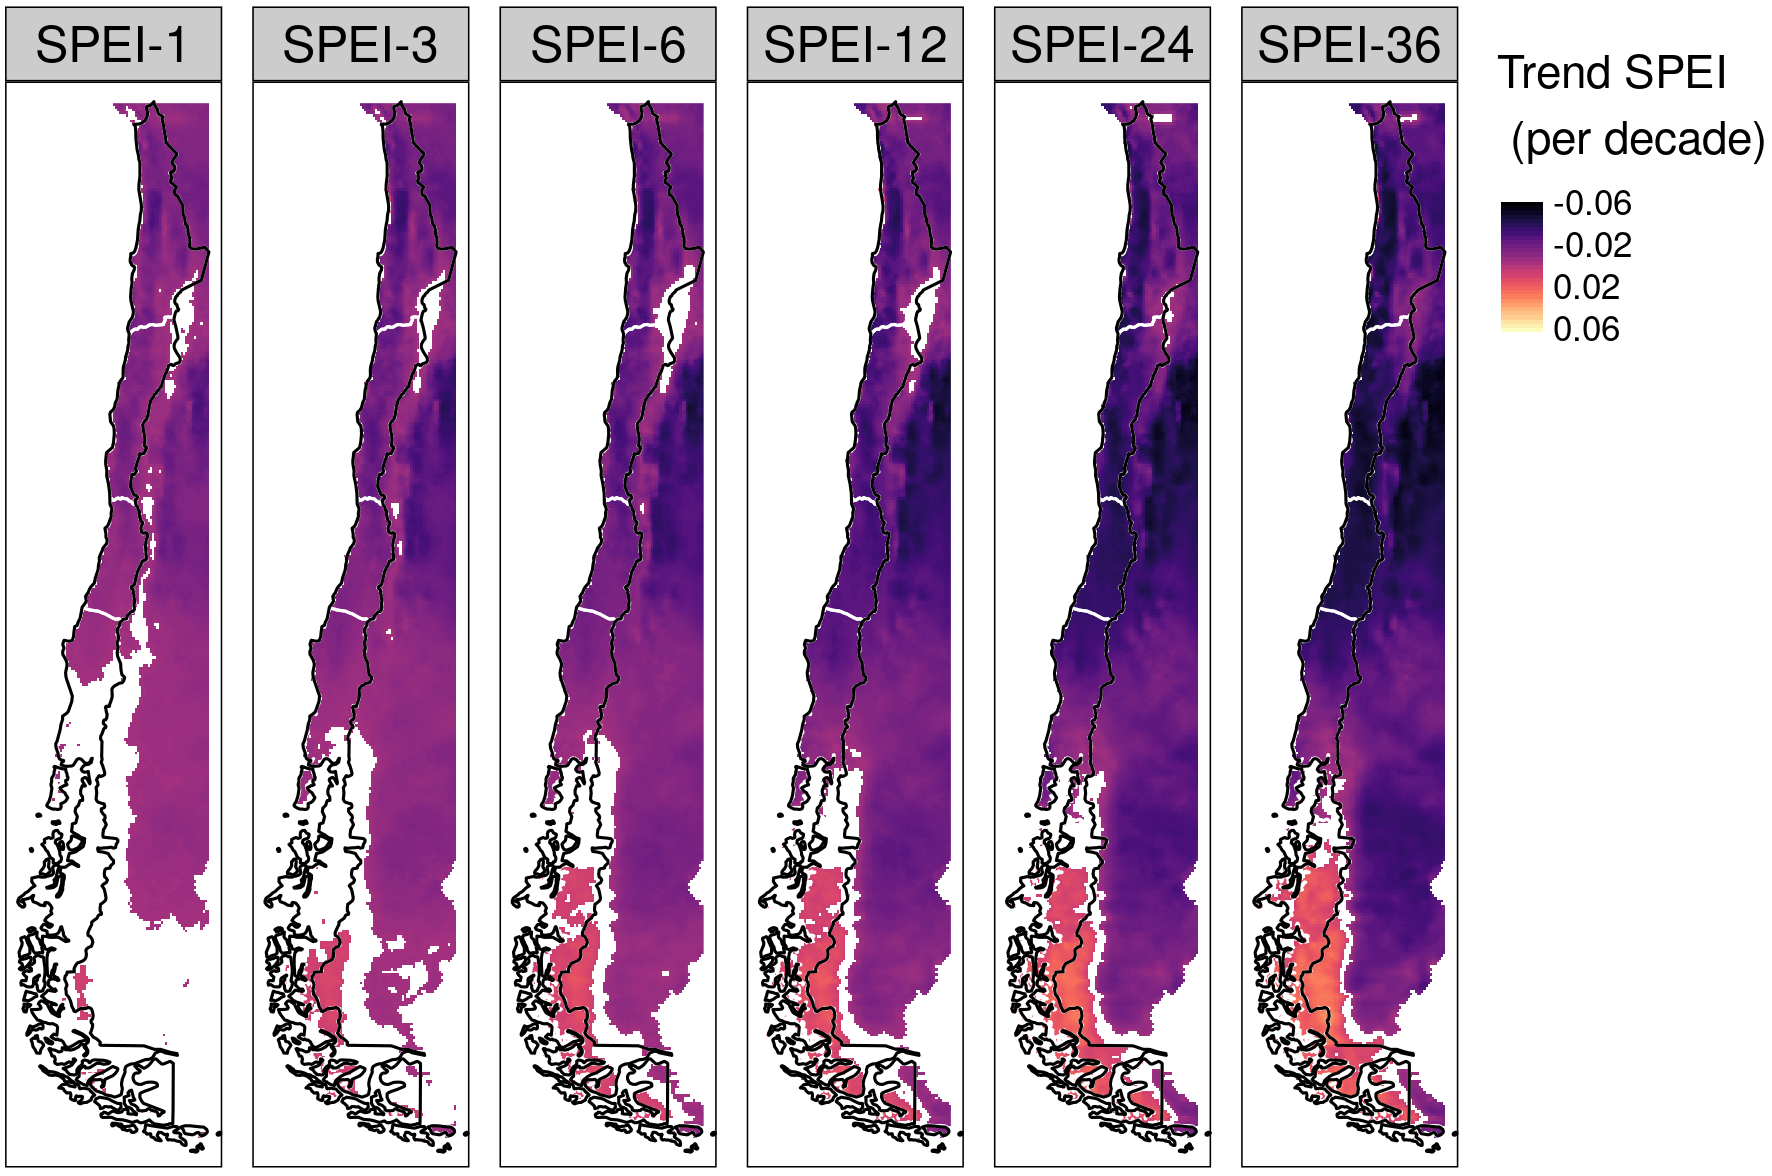
\includegraphics{../output/figs/trend_raster_SPEI_1981-2023.png}

}

}

\subcaption{\label{fig-trendDI-3}SPEI (Standardized Precipitation
Evapotranspiration Index)}
\end{minipage}%
%
\begin{minipage}[t]{0.50\linewidth}

{\centering 

\raisebox{-\height}{

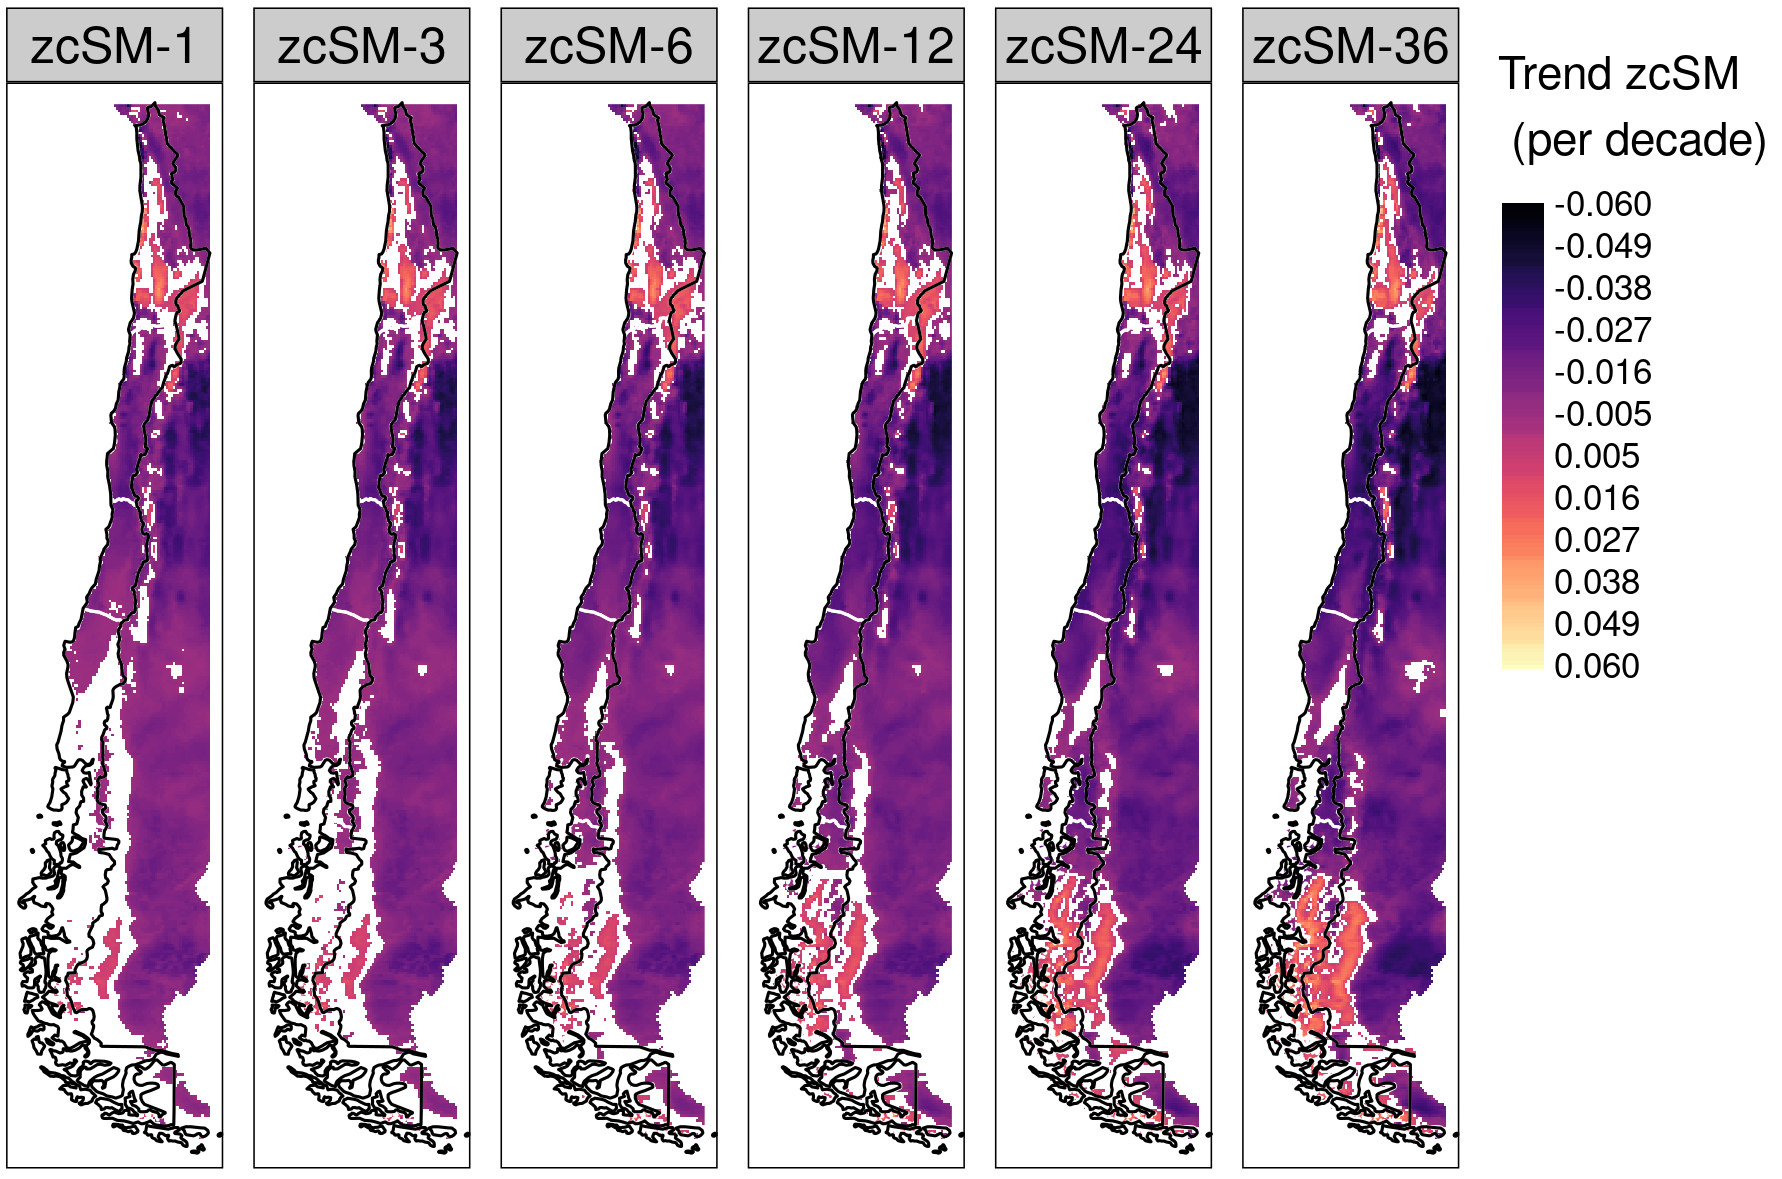
\includegraphics{../output/figs/trend_raster_zcSM_1981-2023.png}

}

}

\subcaption{\label{fig-trendDI-4}SSI (Standardized Soil Moisture Index)}
\end{minipage}%

\caption{\label{fig-trendDI}Linear trend of the drought index (*) at
time scales of 1, 3, 6, 12, 24, and 36 months for 1981-2023}

\end{figure}

\elandscape

\begin{figure}[!ht]

{\centering 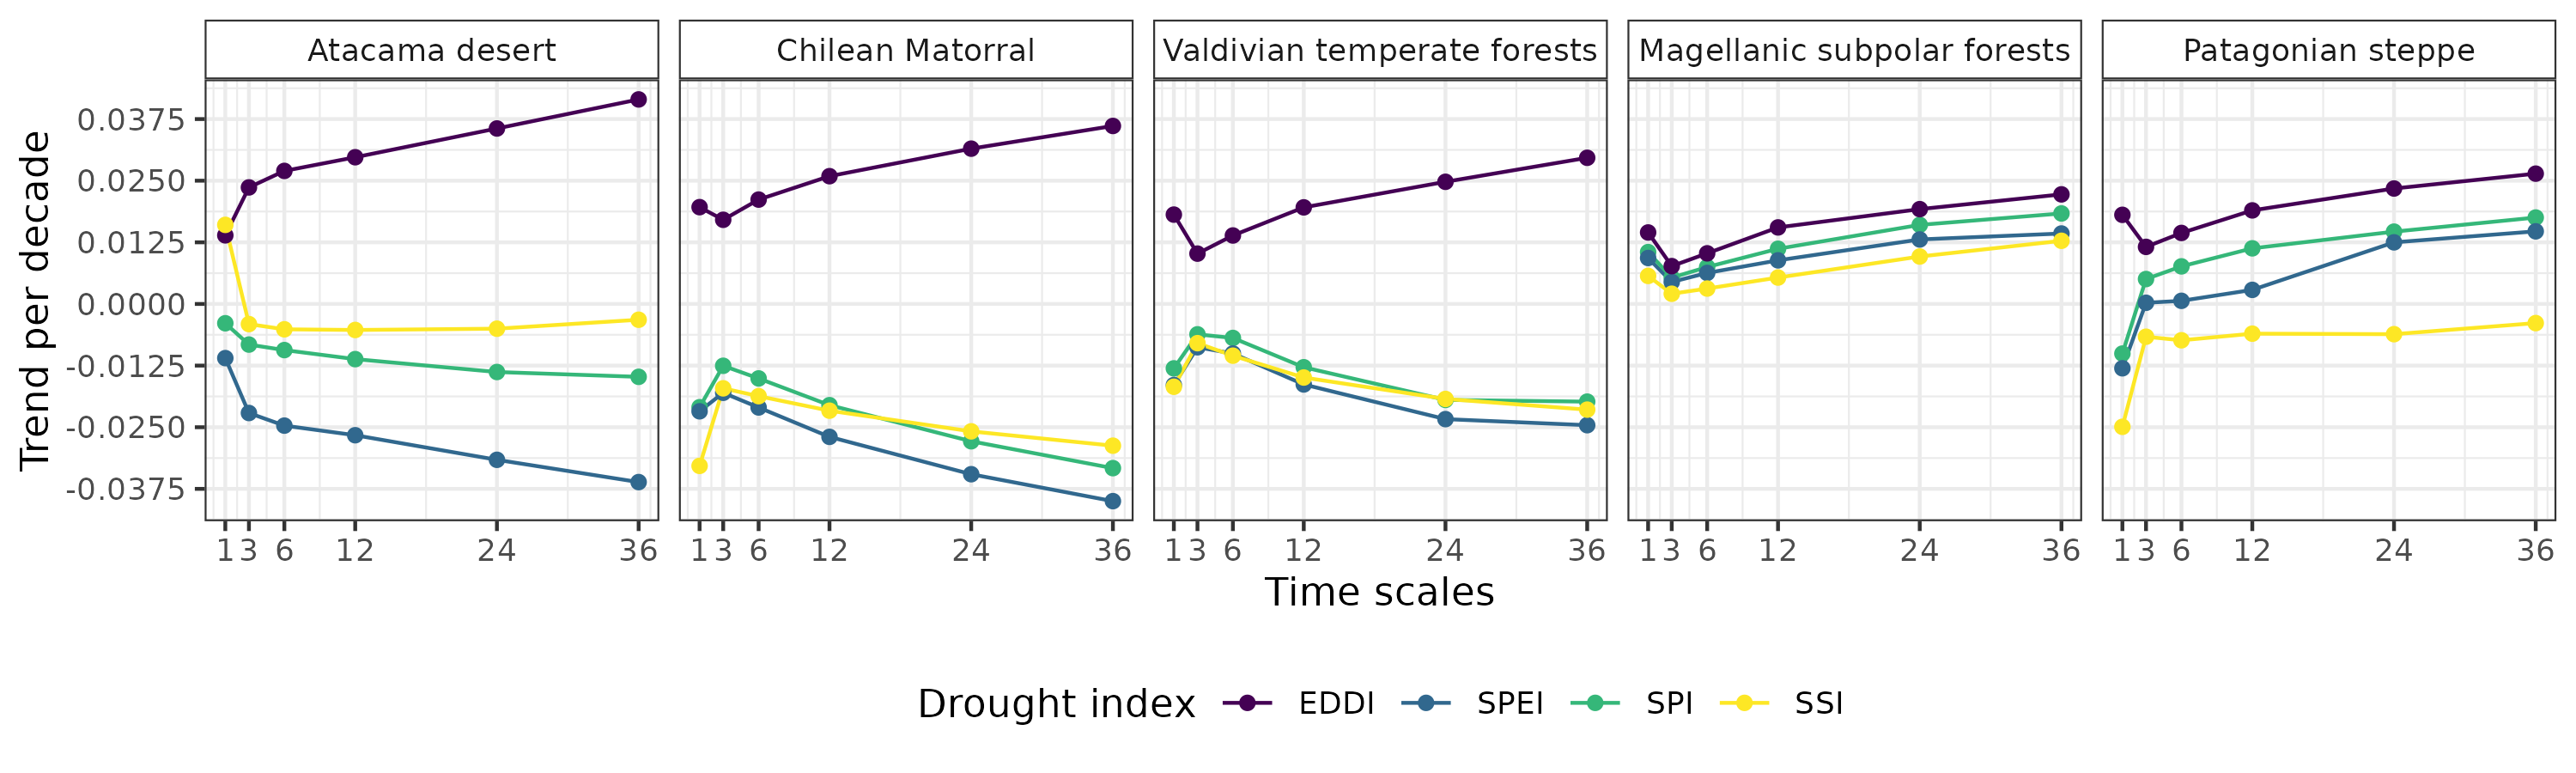
\includegraphics{../output/figs/trend_macrozone_drought_indices.png}

}

\caption{\label{fig-trendDIMacro}Trend per decade for the drought
indices SPI, EDDI, SPEI, and SSI aggregated by macrozone.}

\end{figure}

The Figure~\ref{fig-trendDIMacro} displays the aggregated trend per
macrozone, drought index, and timescale. The macrozones that reached the
lowest trend for SPI, SPEI, and SSI are ``Norte Chico'' and ``Centro'',
where the indices also decrease at longer time scales. This may
potentially be explained by the prolonged reduction in precipitation
that has affected the hydrological system in Chile. At 36 months, it
reaches trends between -0.03 and -0.04 (z-score) per decade for SPI,
SPEI, and SSI. For ``Sur'', the behavior is similar, decreasing at
longer scales and having between -0.016 and -0.025 per decade for SPI,
SPEI, and SSI. ``Norte Grande'' has the highest trend at 36 months for
EDDI (0.042 per decade), and ``Centro'' has the lowest for SPI and SPEI.
In ``Norte Grande'' and ``Norte Chico'', which are in a semi-arid
climate, it is evident that the EDDI has an effect on the difference
between the SPI and SPEI index, which is not seen in the other
macrozones. Contrary to the other macrozones, ``Austral'' showed an
increase in all indices, being the highest for EDDI at 36 months (0.025)
and the lowest for SSI, which shows only a minor increase in the trend.

\hypertarget{interaction-of-land-cover-and-drought-1}{%
\subsection{Interaction of land cover and
drought}\label{interaction-of-land-cover-and-drought-1}}

\hypertarget{land-cover-change-1}{%
\subsubsection{Land cover change}\label{land-cover-change-1}}

\begin{table}[!ht]
\caption{Surface per land cover class that persists during 2001–2022.}
\label{tab-landcoverSurf}
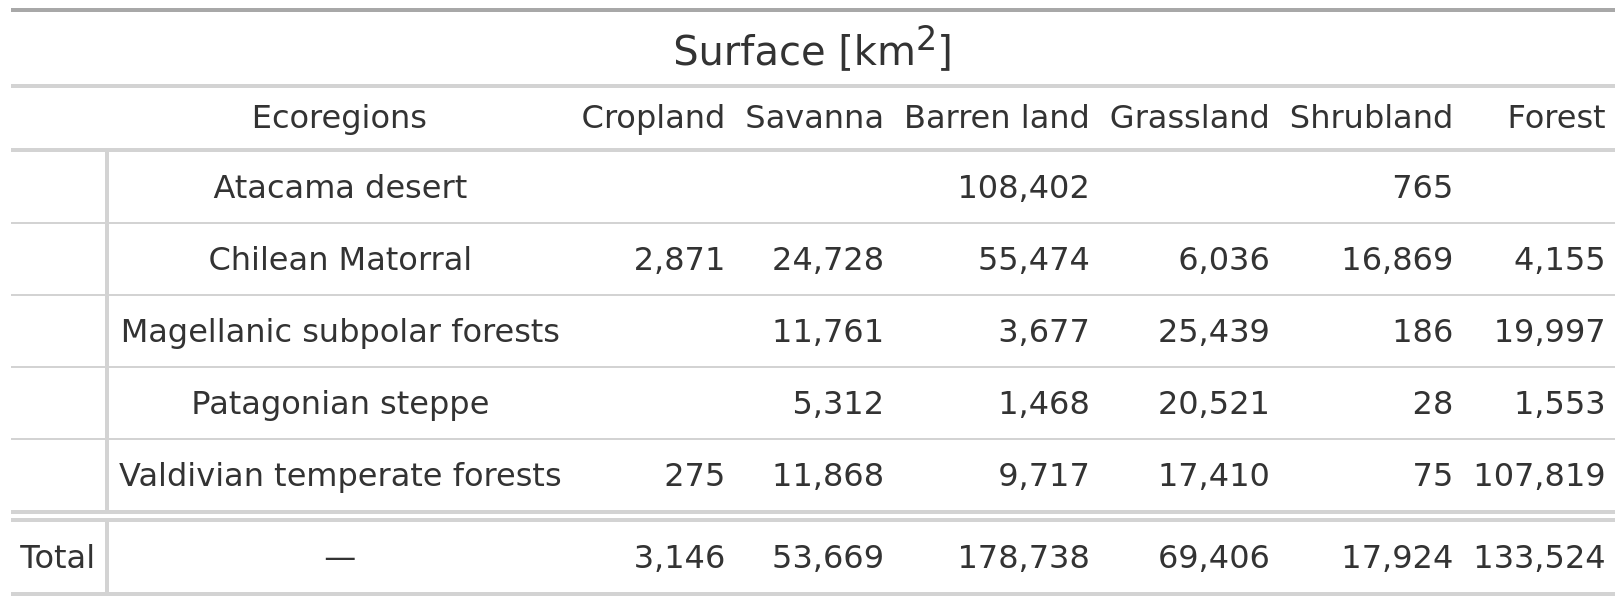
\includegraphics[width = .5\textwidth]{../output/figs/table_surface_landcover_macrozone.png}
\end{table}

\begin{figure}[!ht]

{\centering 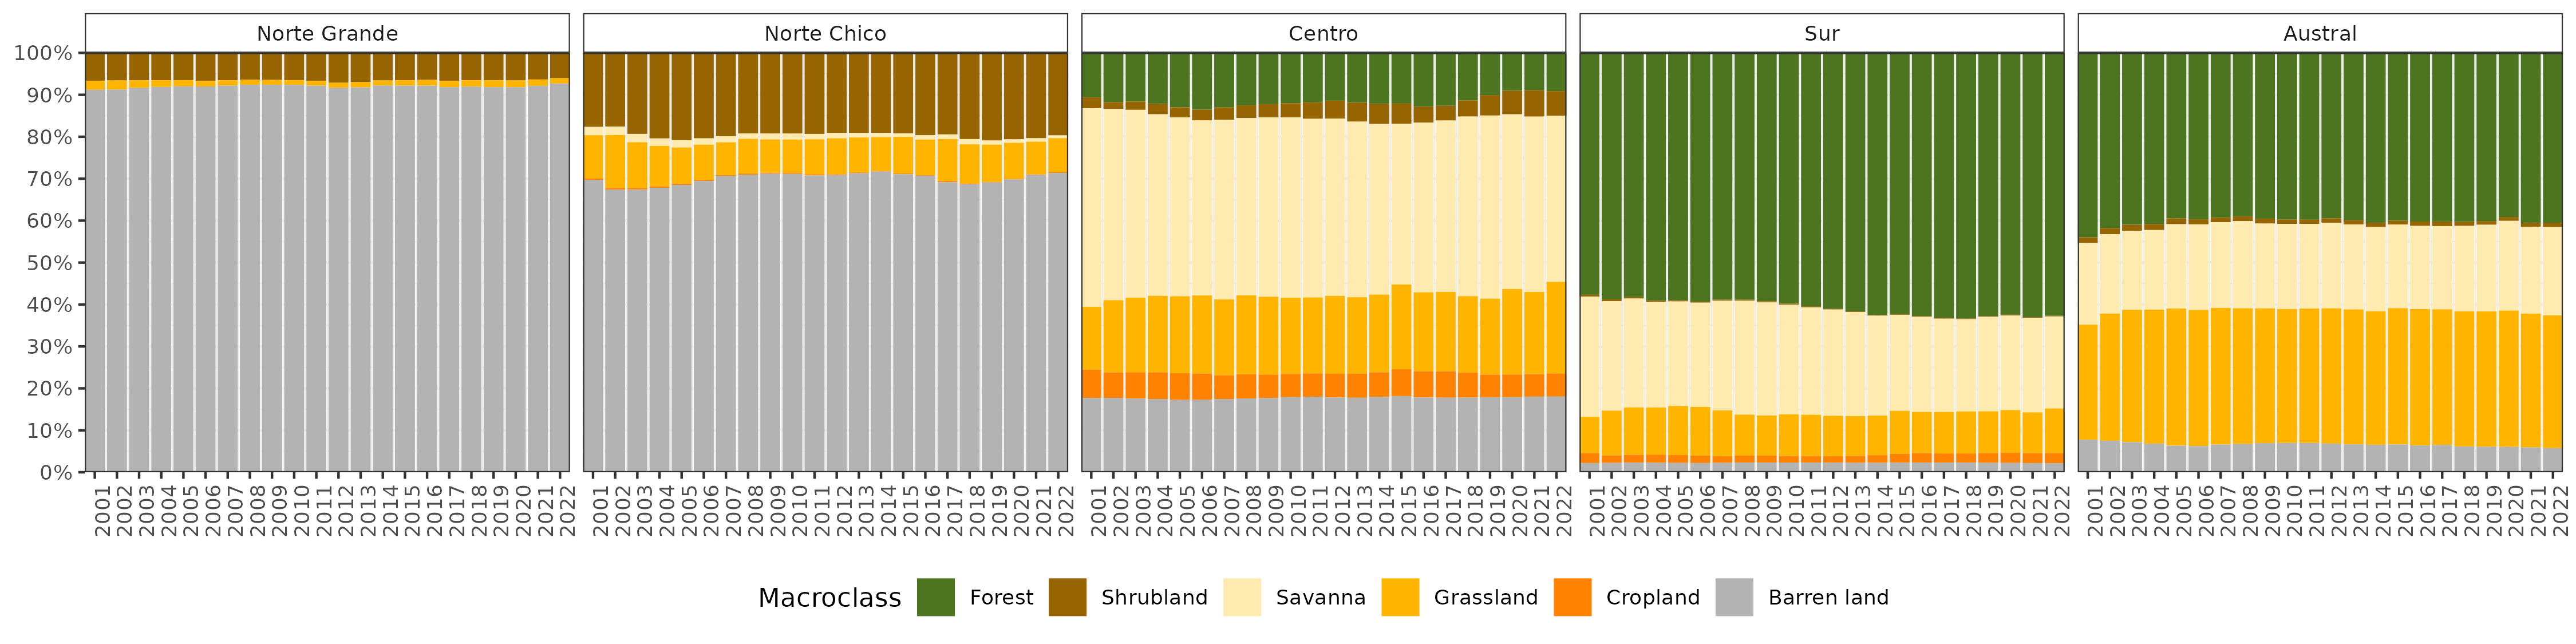
\includegraphics{../output/figs/proportion_landcover_macroclass_2001-2022.png}

}

\caption{\label{fig-LCprop}Proportion of land cover class from the
persistent land cover for 2001-2022 (\textgreater80\%) per macrozone and
land cover macroclass.}

\end{figure}

For vegetation, we obtained and used hereafter five macroclasses of land
cover from IGBP MODIS: forest, shrubland, savanna, grassland, and
croplands. Figure~\ref{fig-studyArea}c shows the spatial distribution of
the macroclasses through Chile for the year 2022.
Figure~\ref{fig-studyArea}d shows the macroclasses of land cover
persistence (80\%) during 2021--2022, respectively (Table
\ref{tab-landcoverSurf}). Within continental Chile, barren land is the
land cover class with the highest surface area (277,870 \(km^2\)). The
largest type of vegetation, with 137,085 \(km^2\), is forest. Grassland
has 74,247 \(km^2\) , savanna 55,206 \(km^2\), shrubland 25,341
\(km^2\), and cropland 3,146 \(km^2\) (Table \ref{tab-landcoverSurf}).
The macrozones with major changes for 2001--2022 were ``Centro'',
``Sur'', and ``Austral'', with 36\%, 31\%, and 34\% of their surface
changing the type of land cover, respectively
(Figure~\ref{fig-studyArea} and Table \ref{tab-landcoverTrend}).
Figure~\ref{fig-LCprop} shows the variation for 2001--2022 in the
proportion of surface per land cover class and macrozone, derived from
the persistence mask over continental Chile.

\begin{table}[!ht]
\caption{The value of Sen's slope trend next to the time-series plot of surface per land cover class (IGBP MCD12Q1.016) for 2001–2022 through Central Chile. Values of zero indicate that there was not a significant trend. The red dots on the plots indicate the maximum and minimum values of the surface. The white cells indicate that the landcover class is not significant in terms of surface area.}
\label{tab-landcoverTrend}
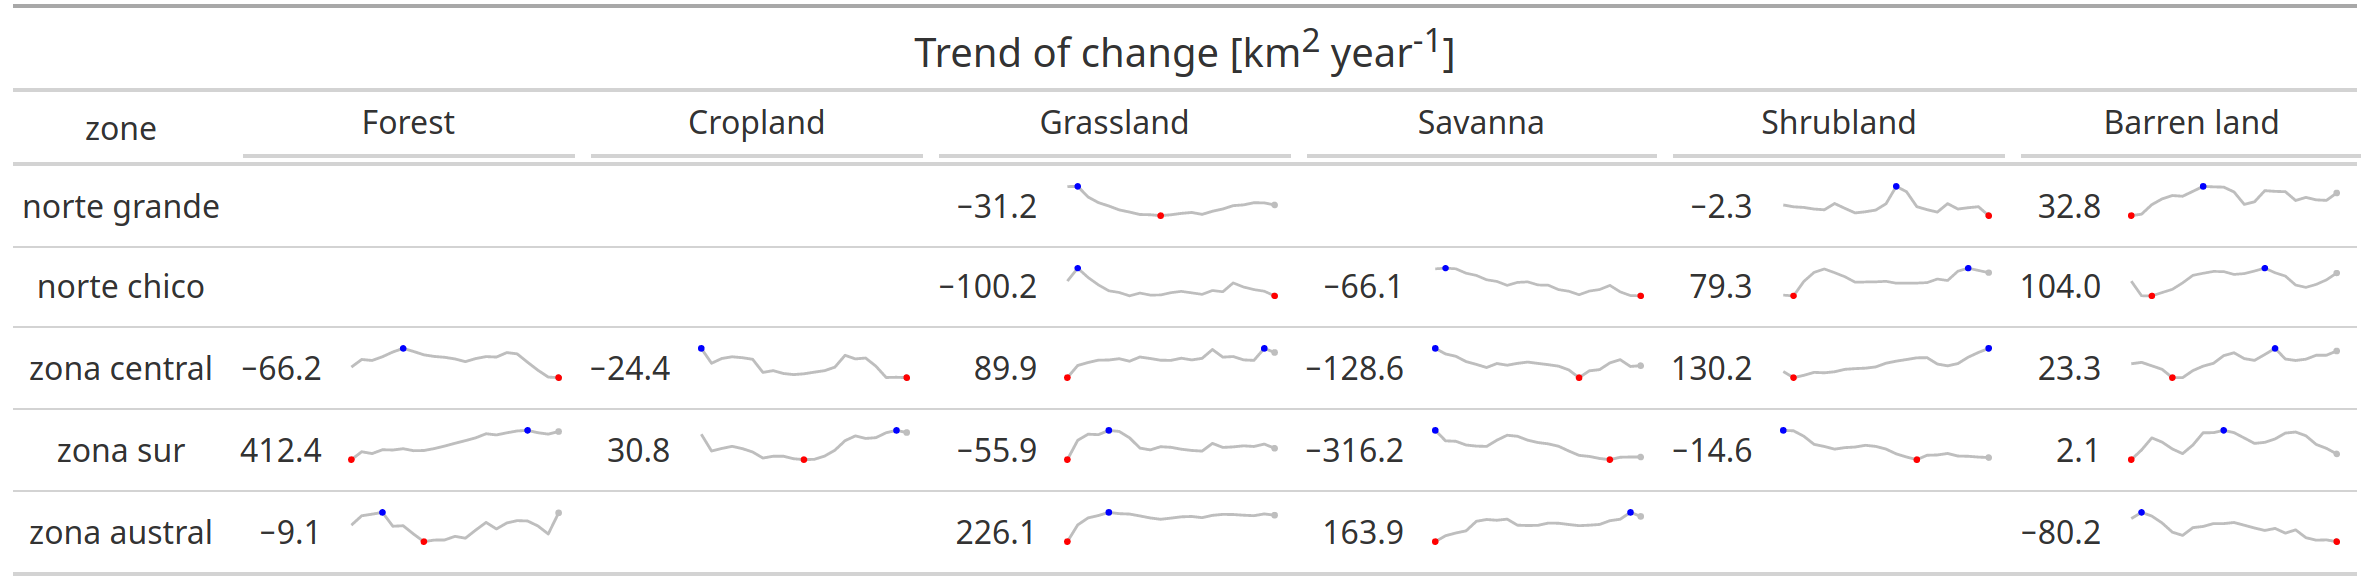
\includegraphics[]{../output/figs/table_var_landcover_macro.png}
\end{table}

From the trend analysis in Table \ref{tab-landcoverTrend}, we can
indicate that the ``Norte Chico'' shows an increase in barren land of
111 \(km^2 yr^{-1}\) and a reduction in the class savanna of 70
\(km^2 yr^{-1}\). In the ``Centro'' and ``Sur'', there are changes with
an important reduction in savanna with 136 and 319 \(km^2 yr^{-1}\),
respectively, and an increase in shrubland and grassland, showing a
change for more dense vegetation types. The area under cultivation
(croplands) appears to be shifting from the ``Centro'' to the ``Sur''.
Also, there is a high increase in forest (397 \(km^2 yr^{-1}\)) in the
``Sur'', seemingly replacing the savanna lost (Table
\ref{tab-landcoverTrend}).

\hypertarget{relationship-between-drought-indices-and-land-cover-change}{%
\subsubsection{Relationship between drought indices and land cover
change}\label{relationship-between-drought-indices-and-land-cover-change}}

\begin{table}[!ht]
\caption{The five most important trends of drought indices in estimating the landcover trend per land cover type and the $R^2$ reached by each random forest model. The white cells indicate that the landcover class is not significant in terms of surface area.}
\label{tab-landcoverTrendRF}
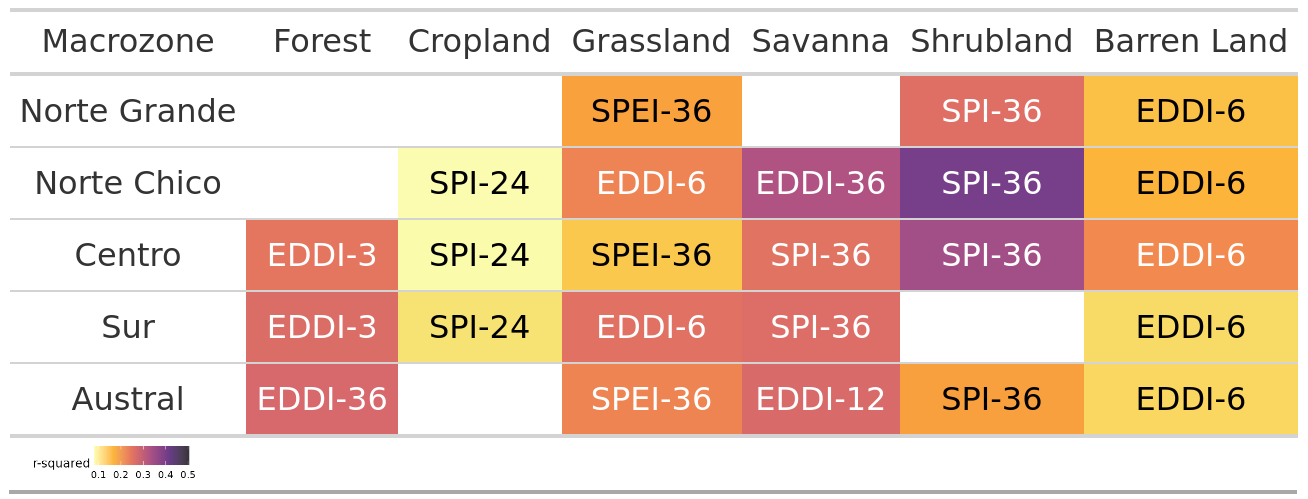
\includegraphics[width=0.5\textwidth]{../output/figs/table_r2_most_important_variables.png}
\end{table}

\begin{figure}[!ht]

{\centering 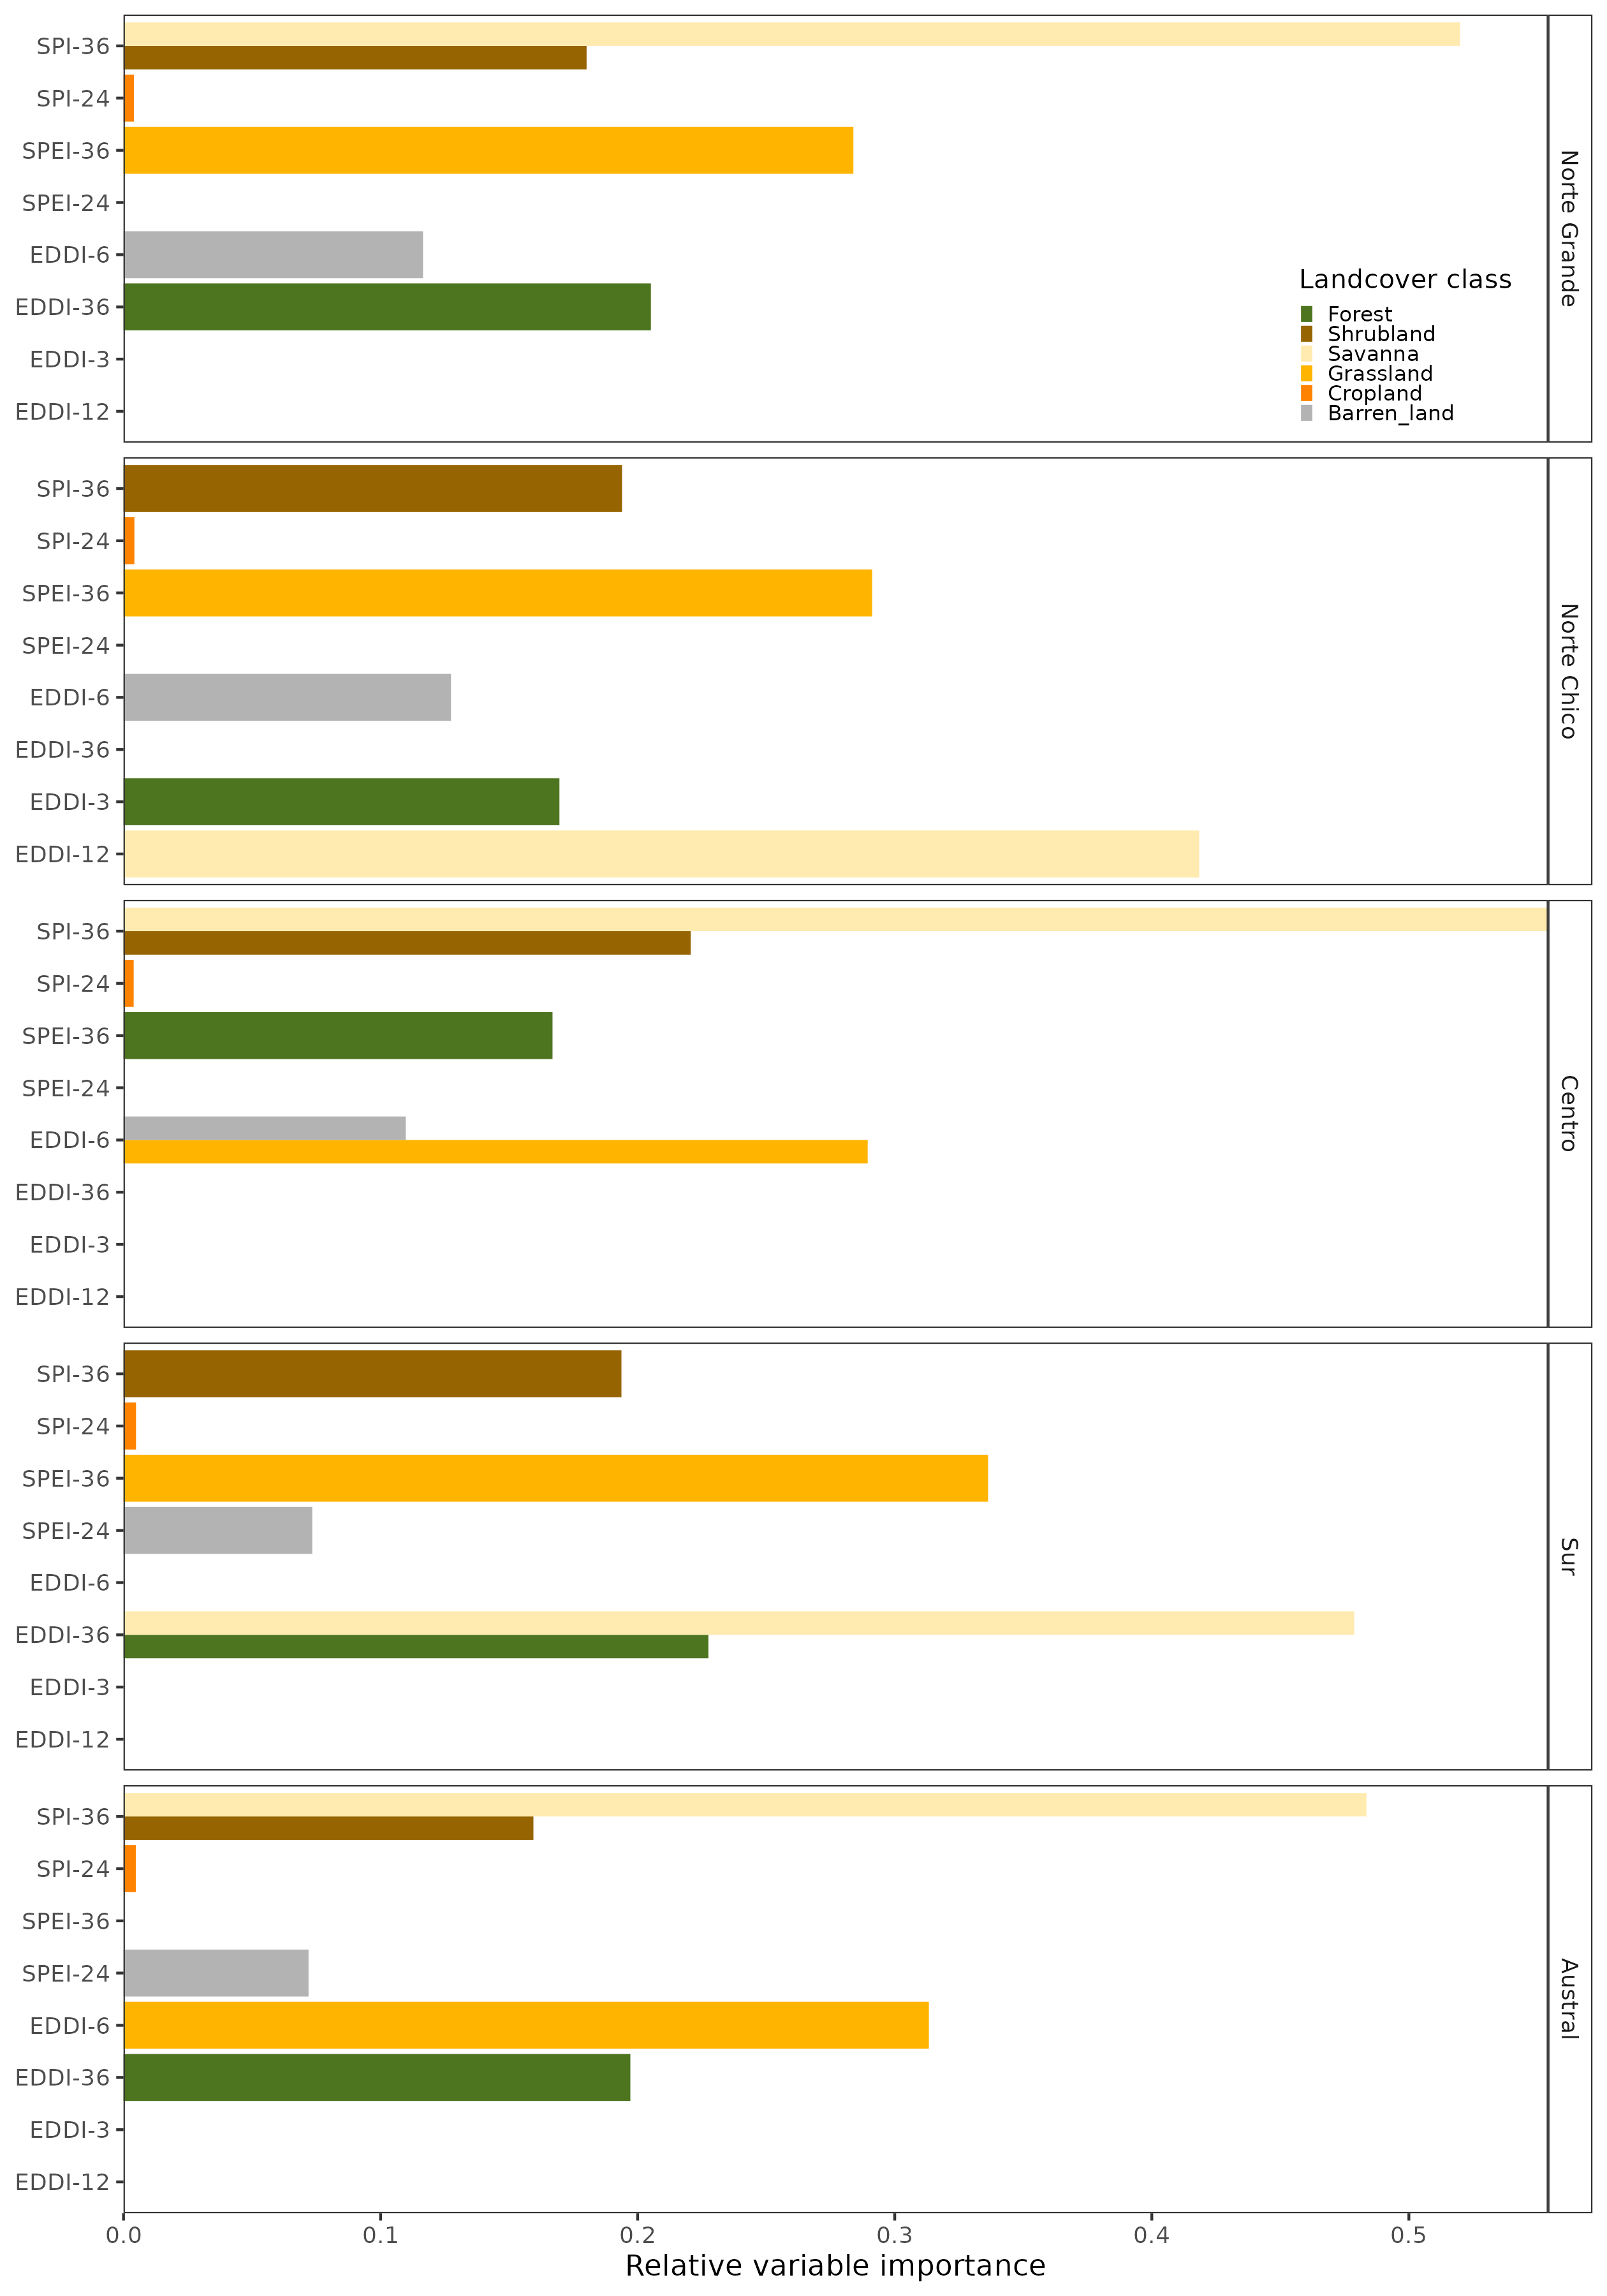
\includegraphics[width=1\textwidth,height=\textheight]{../output/figs/bars_relative_importance_RF.png}

}

\caption{\label{fig-varImportance}Relative importance of drought indices
for explaining the trend in landcover change across the five macrozones
in Chile. SPI, Standardized Precipitation Index; EDDI, Evaporative
Demand Drought Index; SPEI, Standardized Precipitation
Evapotranspiration Index; SSI, Standardized Soil Moisture Index. The
numbers beside the drough index correspond to the time scales.}

\end{figure}

Table \ref{tab-landcoverTrendRF} shows the drought indices that are the
most important variables in the random forest models, together with the
\(R^2\) reached. The random forest models reached an \(R^2\) between
0.12 and 0.41 for the land cover types and macrozones. The model shows
the highest \(R^2\) for shrublands (0.28 to 0.42) and the lowest \(R^2\)
for croplands (0.16 to 0.20) across all macrozones.

Figure~\ref{fig-varImportance} shows the three most important variables
for the models across the five macrozones and per landcover type. For
shurublands, the SPI of long-term and short-term SSI were the most
relevant drought indices within the five macrozones. We showed that the
trend in short-term EDDI (1--6 months) and long-term SPI (24- and
36-months) affected grasslands and forest changes. We showed that trends
in SPI-36 and long-term trends in EDDI (12 to 36 months) were associated
with changes in savannas. The changes in barren land are shown to be
limited to the changes in the short-term AED (1 to 6 months). Changes in
croplands have not been linked to drought across all macrozones. The
supplementary material in Section S3 provides further details about the
variable's importance.

\begin{figure}[!ht]

{\centering 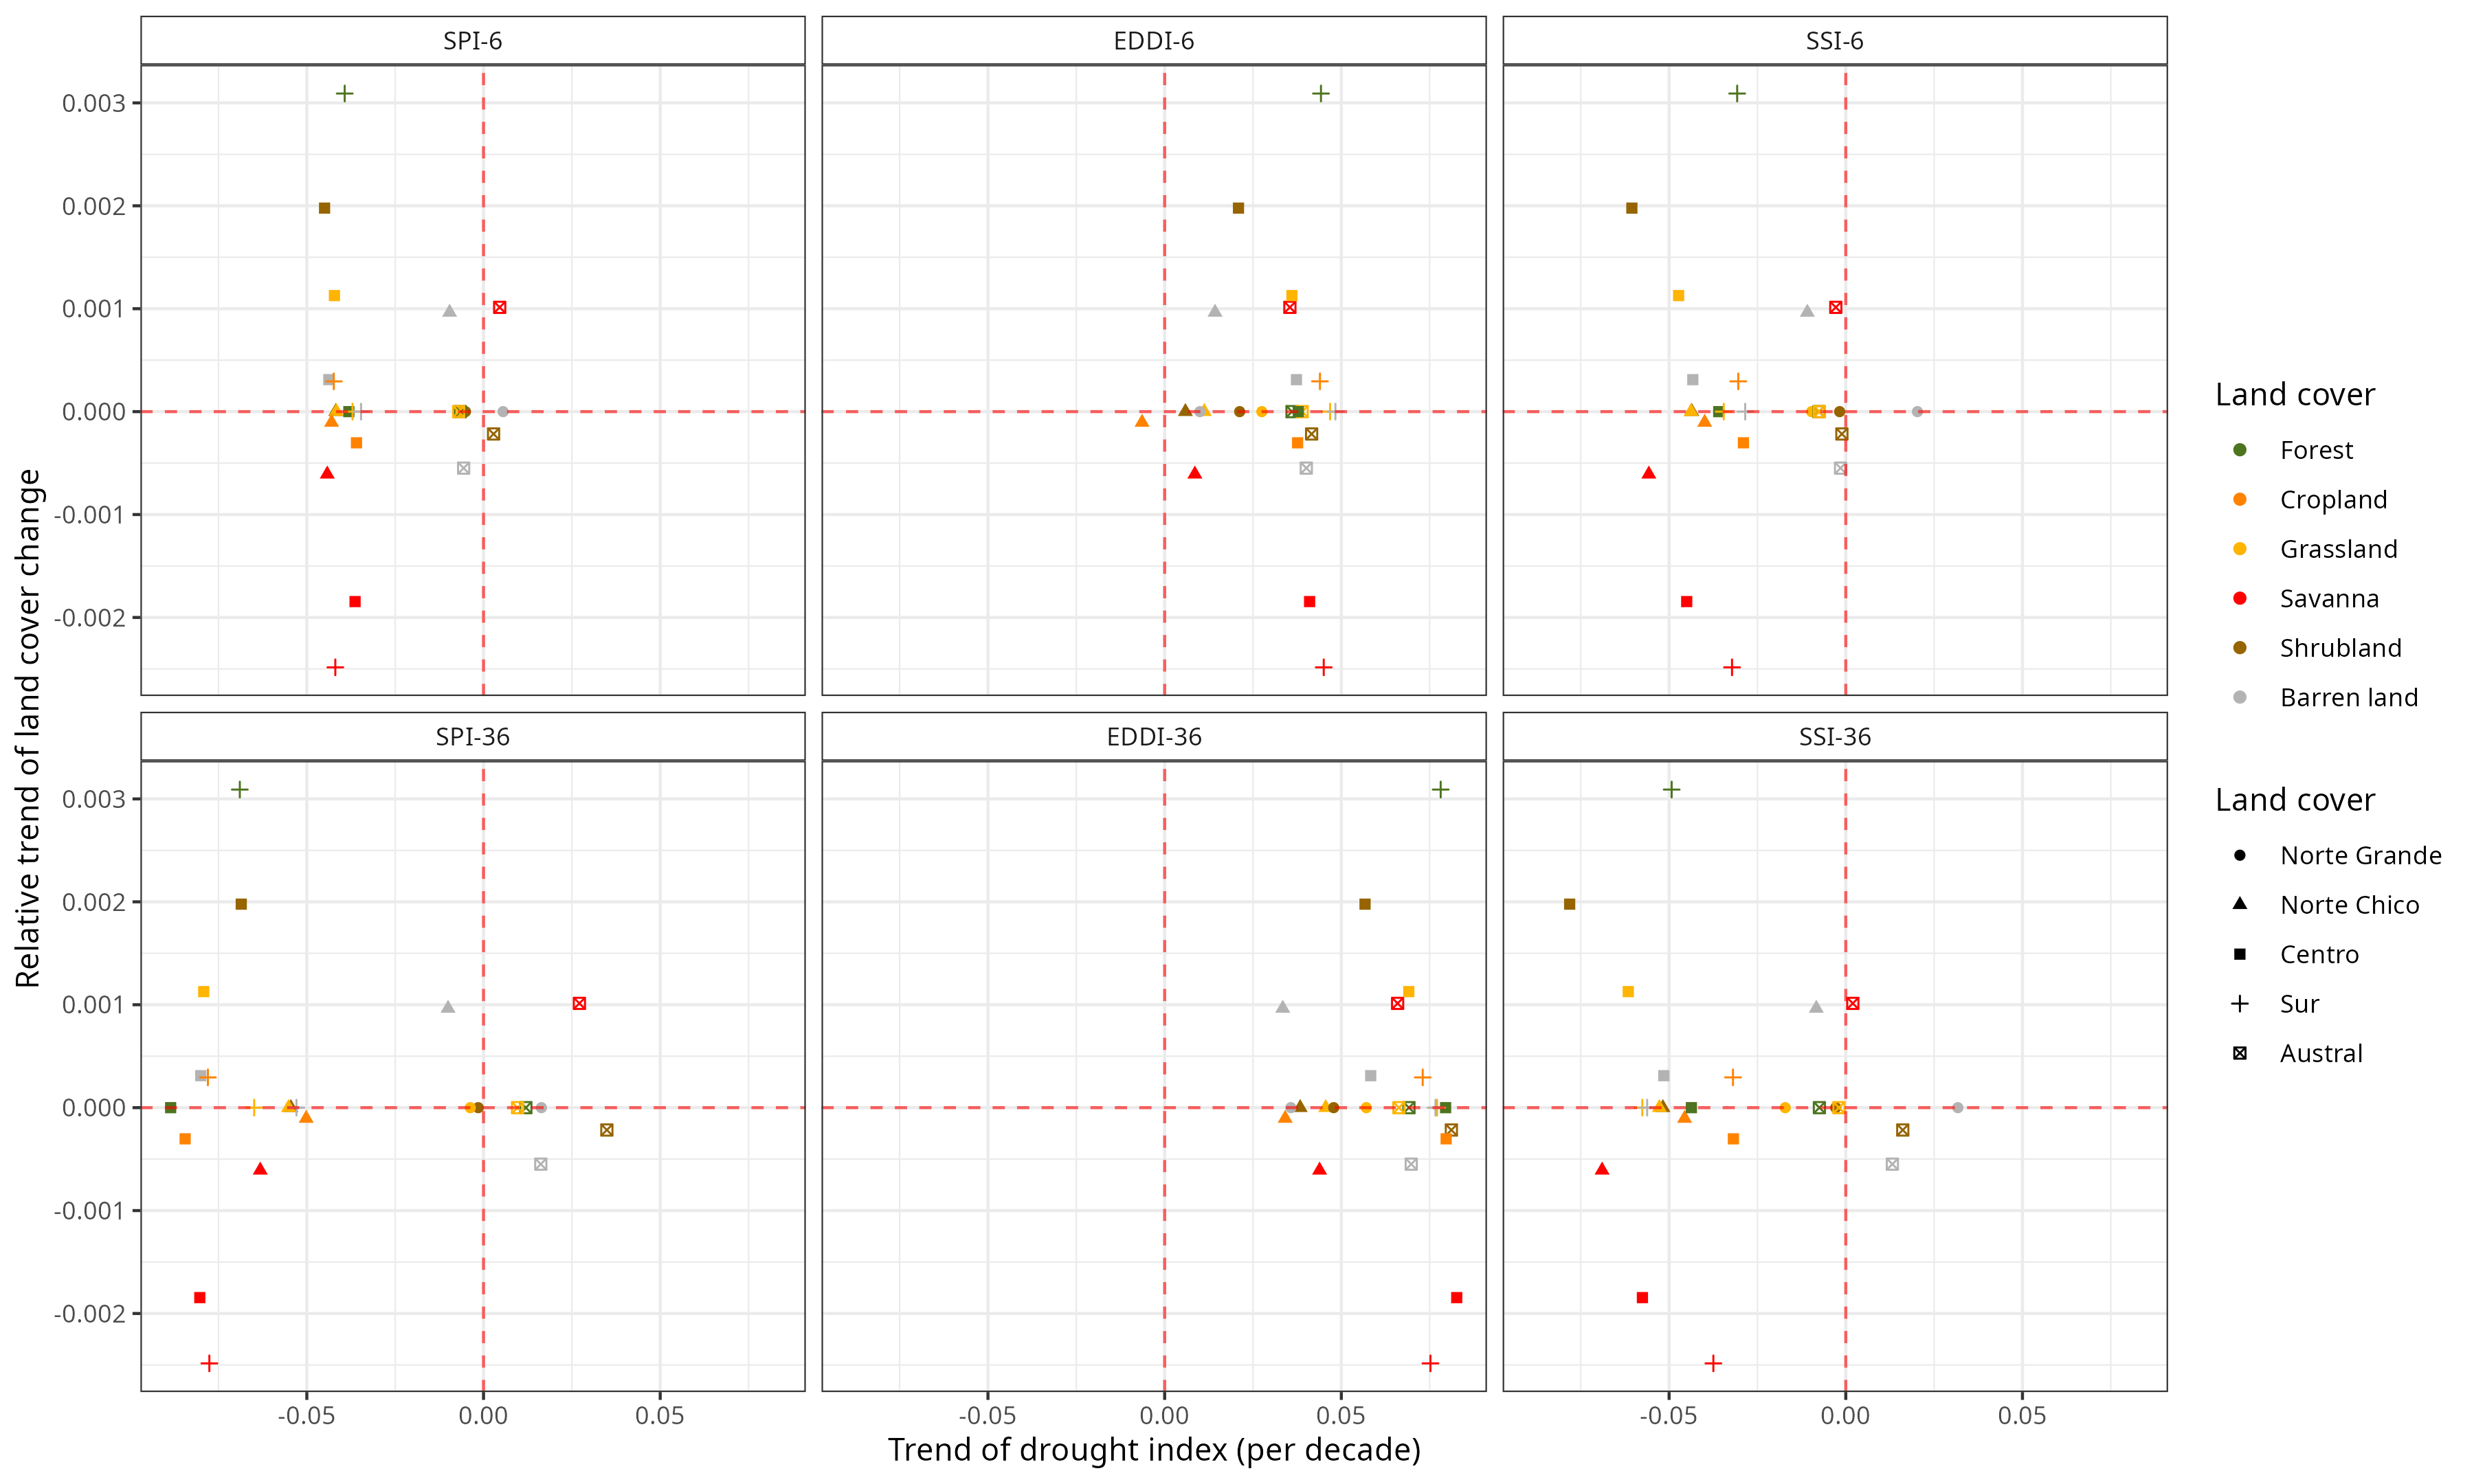
\includegraphics{../output/figs/points_landcover_drought_indices_trend_and_time_scale.png}

}

\caption{\label{fig-TrendsLandDrought}Relationship between the trend in
land cover change (y-axis) and the trend in drought indices (x-axis) for
the five macrozones. Vertical panels correspond to short (6 months) and
long (36 months) time scales. Horizontal panels show the drought indices
SPI, EDDI, and SSI.}

\end{figure}

Figure~\ref{fig-TrendsLandDrought} shows the connection between the SPI,
EDDI, and SSI drought indices for time scales of 6 and 36 months against
changes in land cover. Forest in the ``Sur'', shrubland and grassland in
``Centro'', barren land in ``Norte Chico'', and savanna in ``Austral''
showed an increase in land cover extent, which was associated with an
increase in EDDI. Savanna in ``Centro'', ``Sur'', and ``Norte Chico''
decreases with the increase in EDDI. The SPI and SSI showed similar
behavior regarding the trend in land cover type. A decrease in SPI and
SSI is associated with an increase in the surface in shrubland and
grassland in ``Centro'', forest in ``Sur'', and barren land in ``Norte
Chico'', as well as a decrease trend in savanna in ``Norte Chico'',
``Centro'', and ``Sur''.

\hypertarget{drought-impacts-on-vegetation-productivity-within-land-cover}{%
\subsection{Drought impacts on vegetation productivity within land
cover}\label{drought-impacts-on-vegetation-productivity-within-land-cover}}

\hypertarget{trends-in-vegetation-productivity}{%
\subsubsection{Trends in vegetation
productivity}\label{trends-in-vegetation-productivity}}

\begin{figure}[!ht]

{\centering 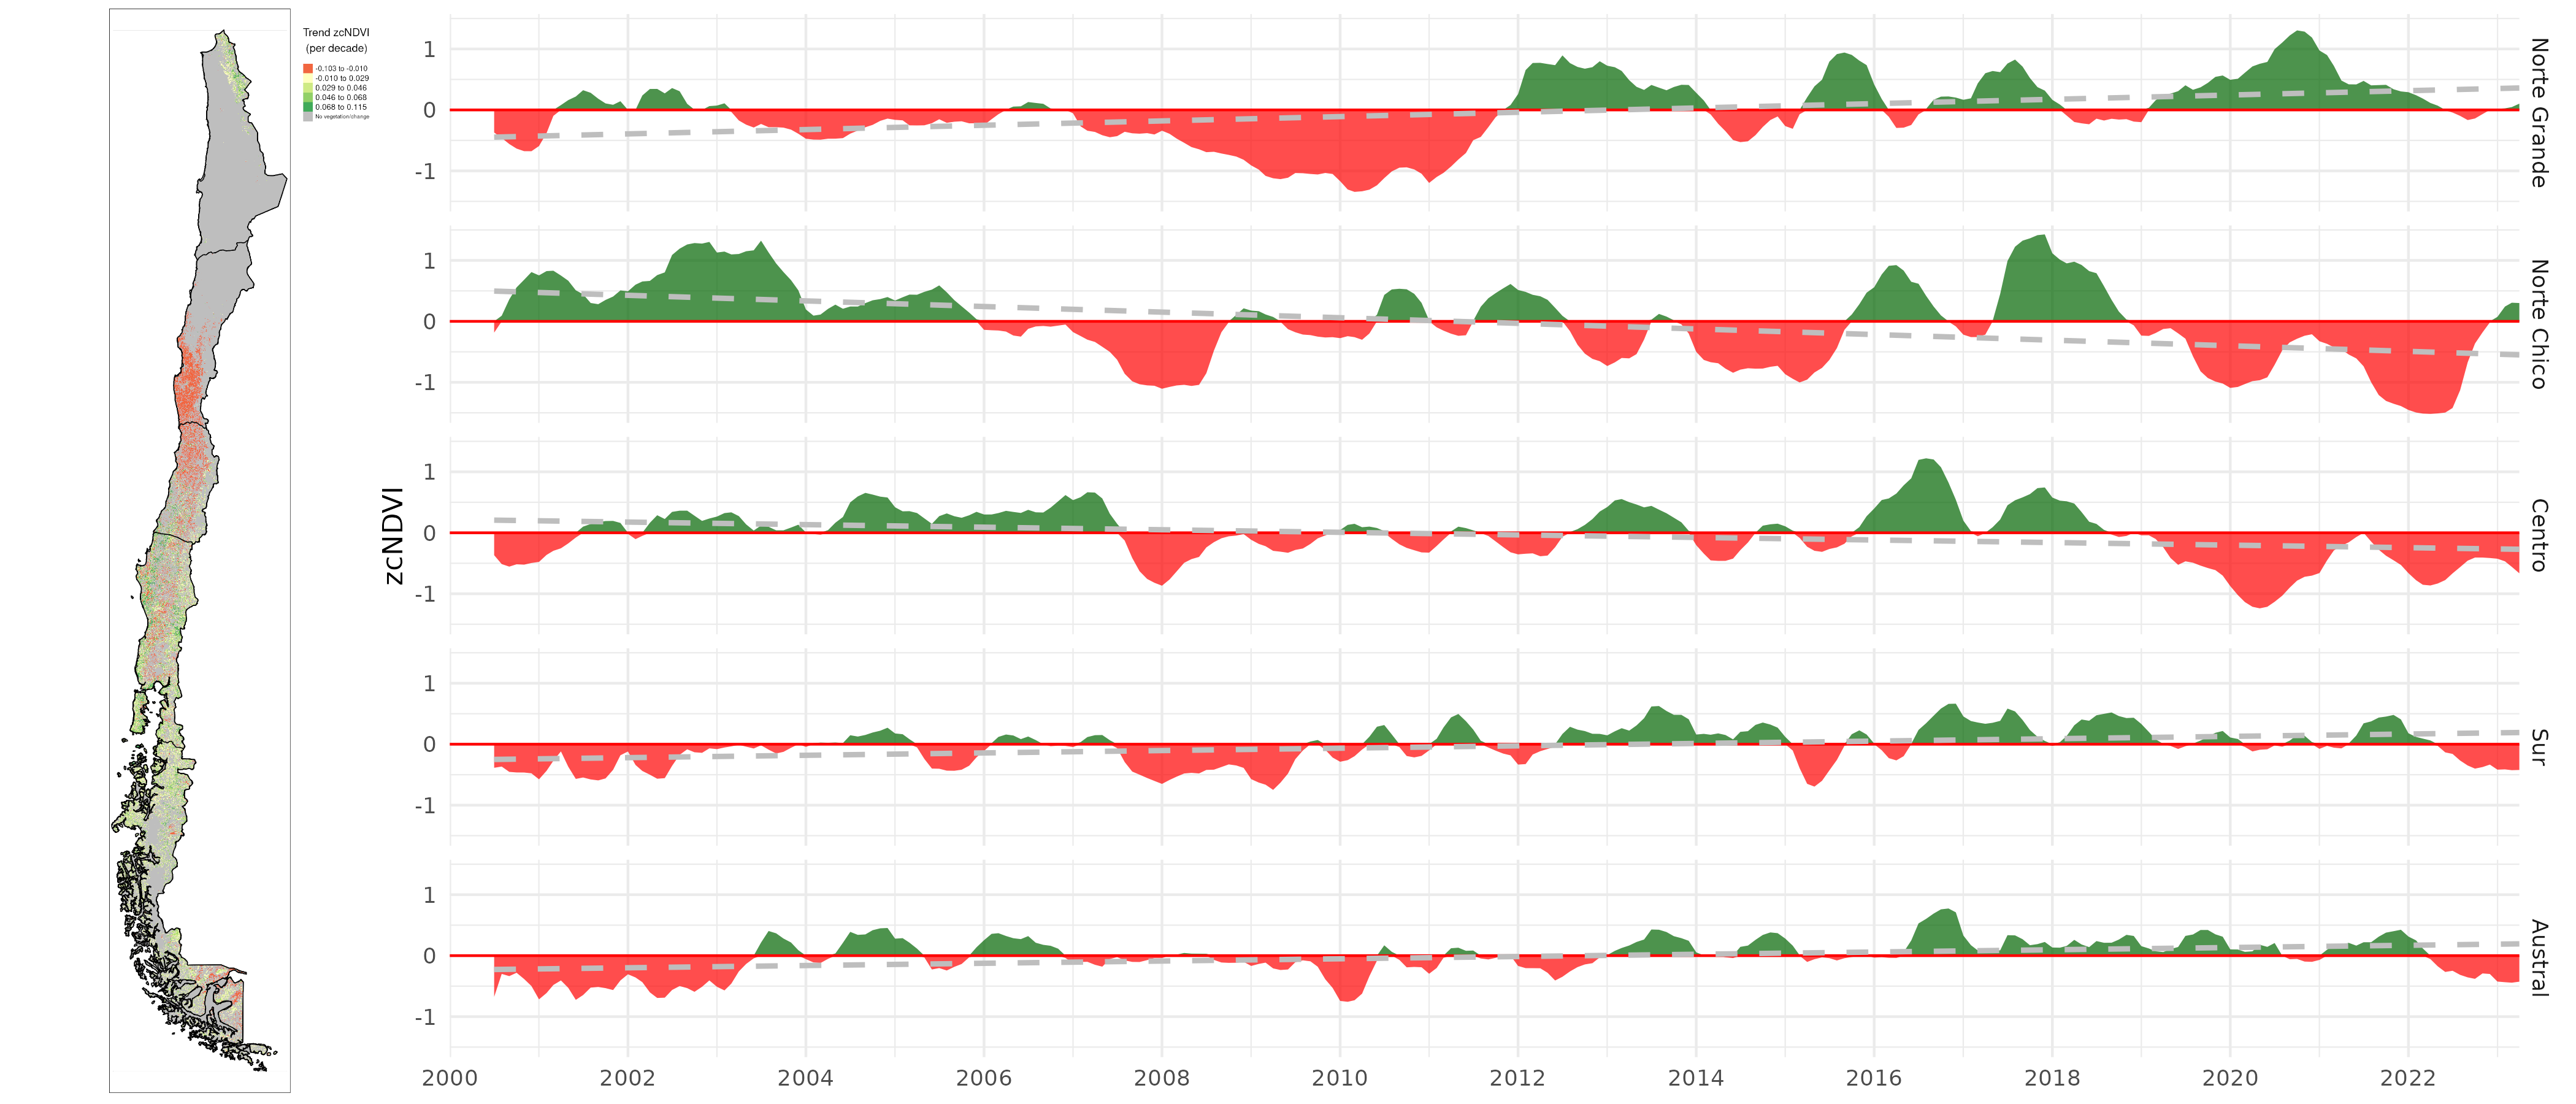
\includegraphics{../output/figs/temporal_variation_zcNDVI6_macrozonas_con_mapa.png}

}

\caption{\label{fig-zcNDVI_var}(a) Map of the linear trend of the index
zcNDVI for 2000--2023. Greener colors indicate a positive trend; reder
colors correspond to a negative trend and a decrease in vegetation
productivity. Grey colors indicate either no vegetation or a change in
land cover type for 2001--2022. (b) Temporal variation of zcNDVI
aggregated at macrozone level within continental Chile. Each horizontal
panel corresponds to a macrozone from `Norte Grande' to `Austral'.}

\end{figure}

Figure~\ref{fig-zcNDVI_var} shows a spatial map of trends in zcNDVI
(Figure~\ref{fig-zcNDVI_var}a). In ``Norte Grande'', vegetation
productivity, as per the z-index, exhibits a yearly increase of 0.027
for grassland and 0.032 for shrubland. In ``Norte Chico'', savanna has
the lowest trend slope of -0.062, cropland -0.047, shrubland -0.042, and
grassland -0.037. In ``Centro'', shrubland reaches -0.07, savanna
-0.031, cropland -0.024, forest -0.017, and grassland -0.005 per decade.
This decrease in productivity could be associated either with a
reduction in vegetation surface, a decrease in biomass, or browning.

The temporal variation within the macrozones is shown in
Figure~\ref{fig-zcNDVI_var}b. There is a negative trend in ``Norte
Chico'' with -0.035 and ``Centro'' with -0.02 per decade. Vegetation
reached its lowest values for 2019-2022, with an extreme condition in
early 2020 and 2022 in the ``Norte Chico'' and ``Centro''. The ``Sur''
and ``Austral'' show a positive trend of around 0.012 and 0.016,
respectively, per decade (Figure~\ref{fig-zcNDVI_var}).

\hypertarget{correlation-between-vegetation-productivity-and-drought-indices}{%
\subsubsection{Correlation between vegetation productivity and drought
indices}\label{correlation-between-vegetation-productivity-and-drought-indices}}

\begin{figure}[!ht]

{\centering 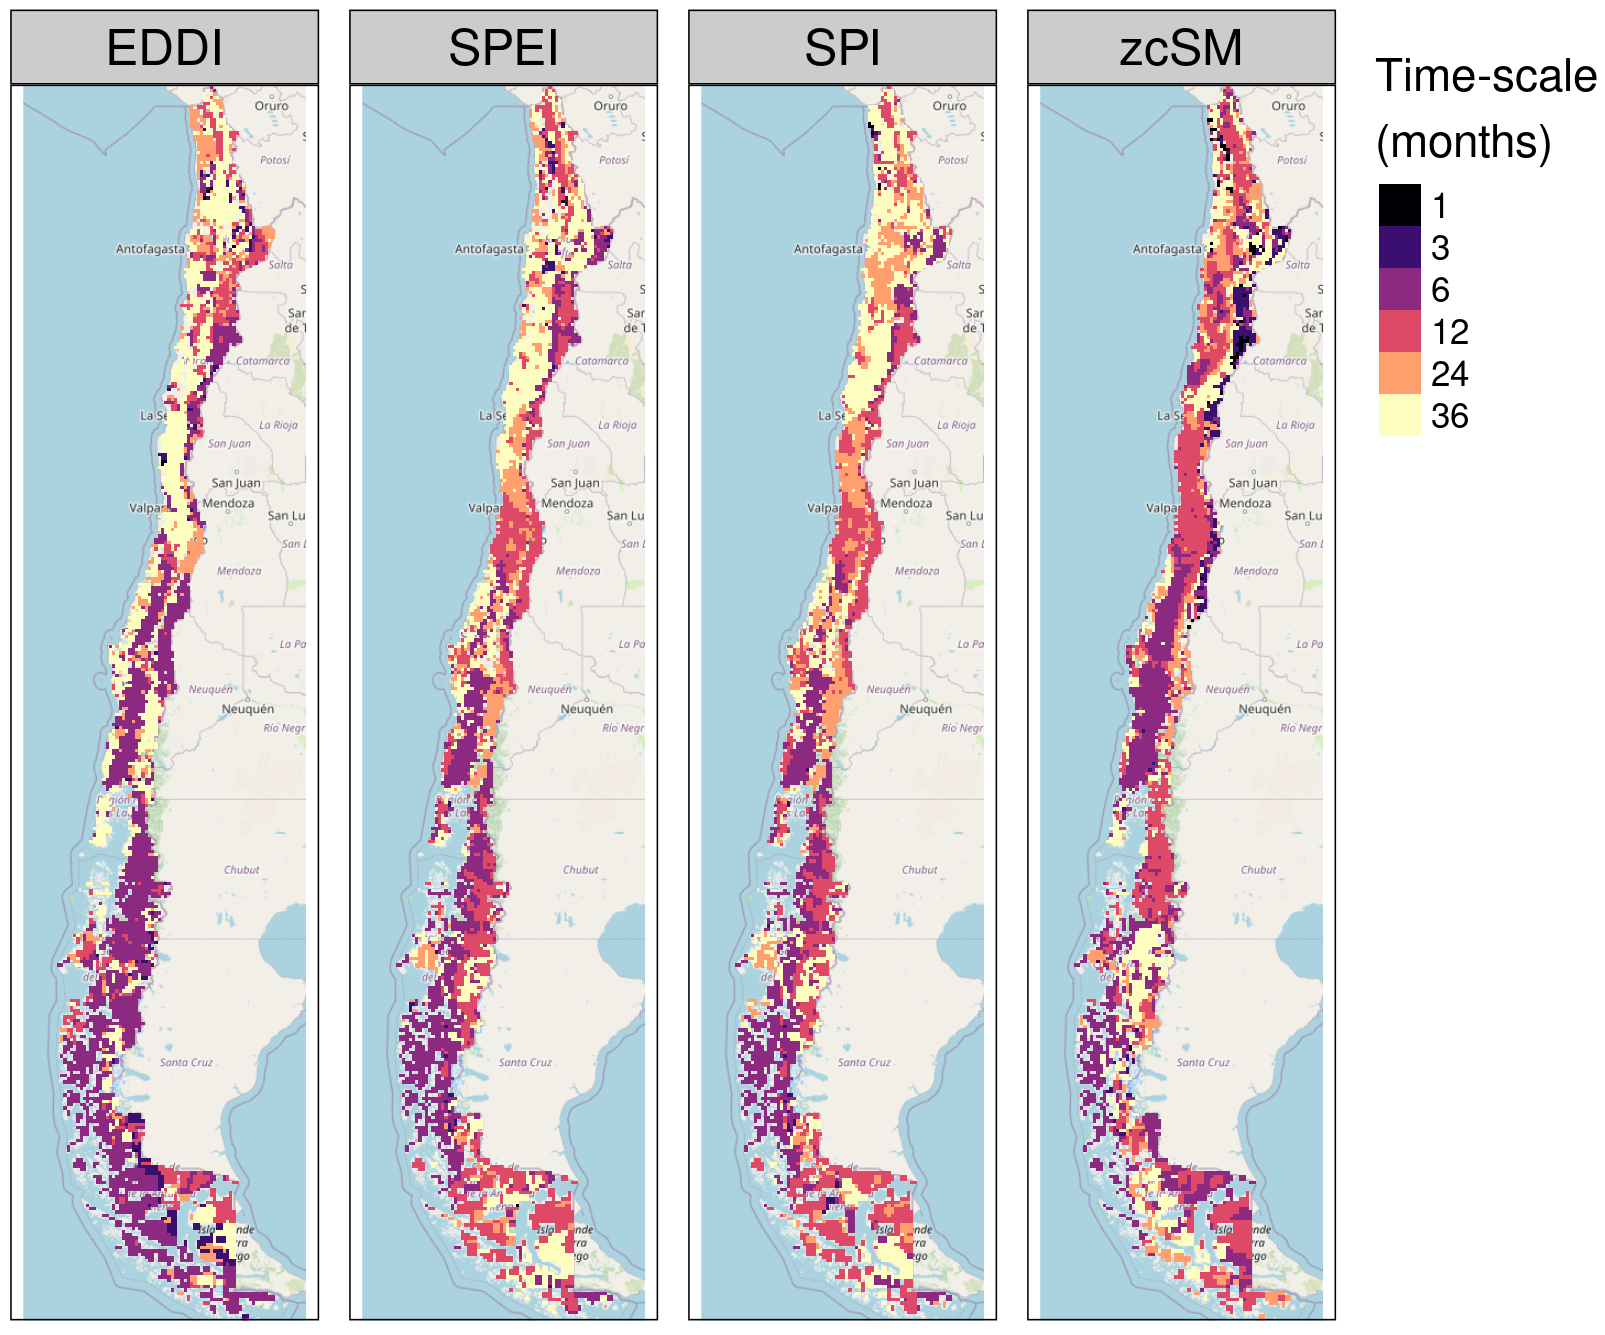
\includegraphics{../output/figs/mapa_cor_selec_indices_zcNDVI6.png}

}

\caption{\label{fig-corTimeScale}Time scales per drought index that
reach the maximum coefficient of determination. White spaces indicate no
significant correlation.}

\end{figure}

\begin{figure}[!ht]

{\centering 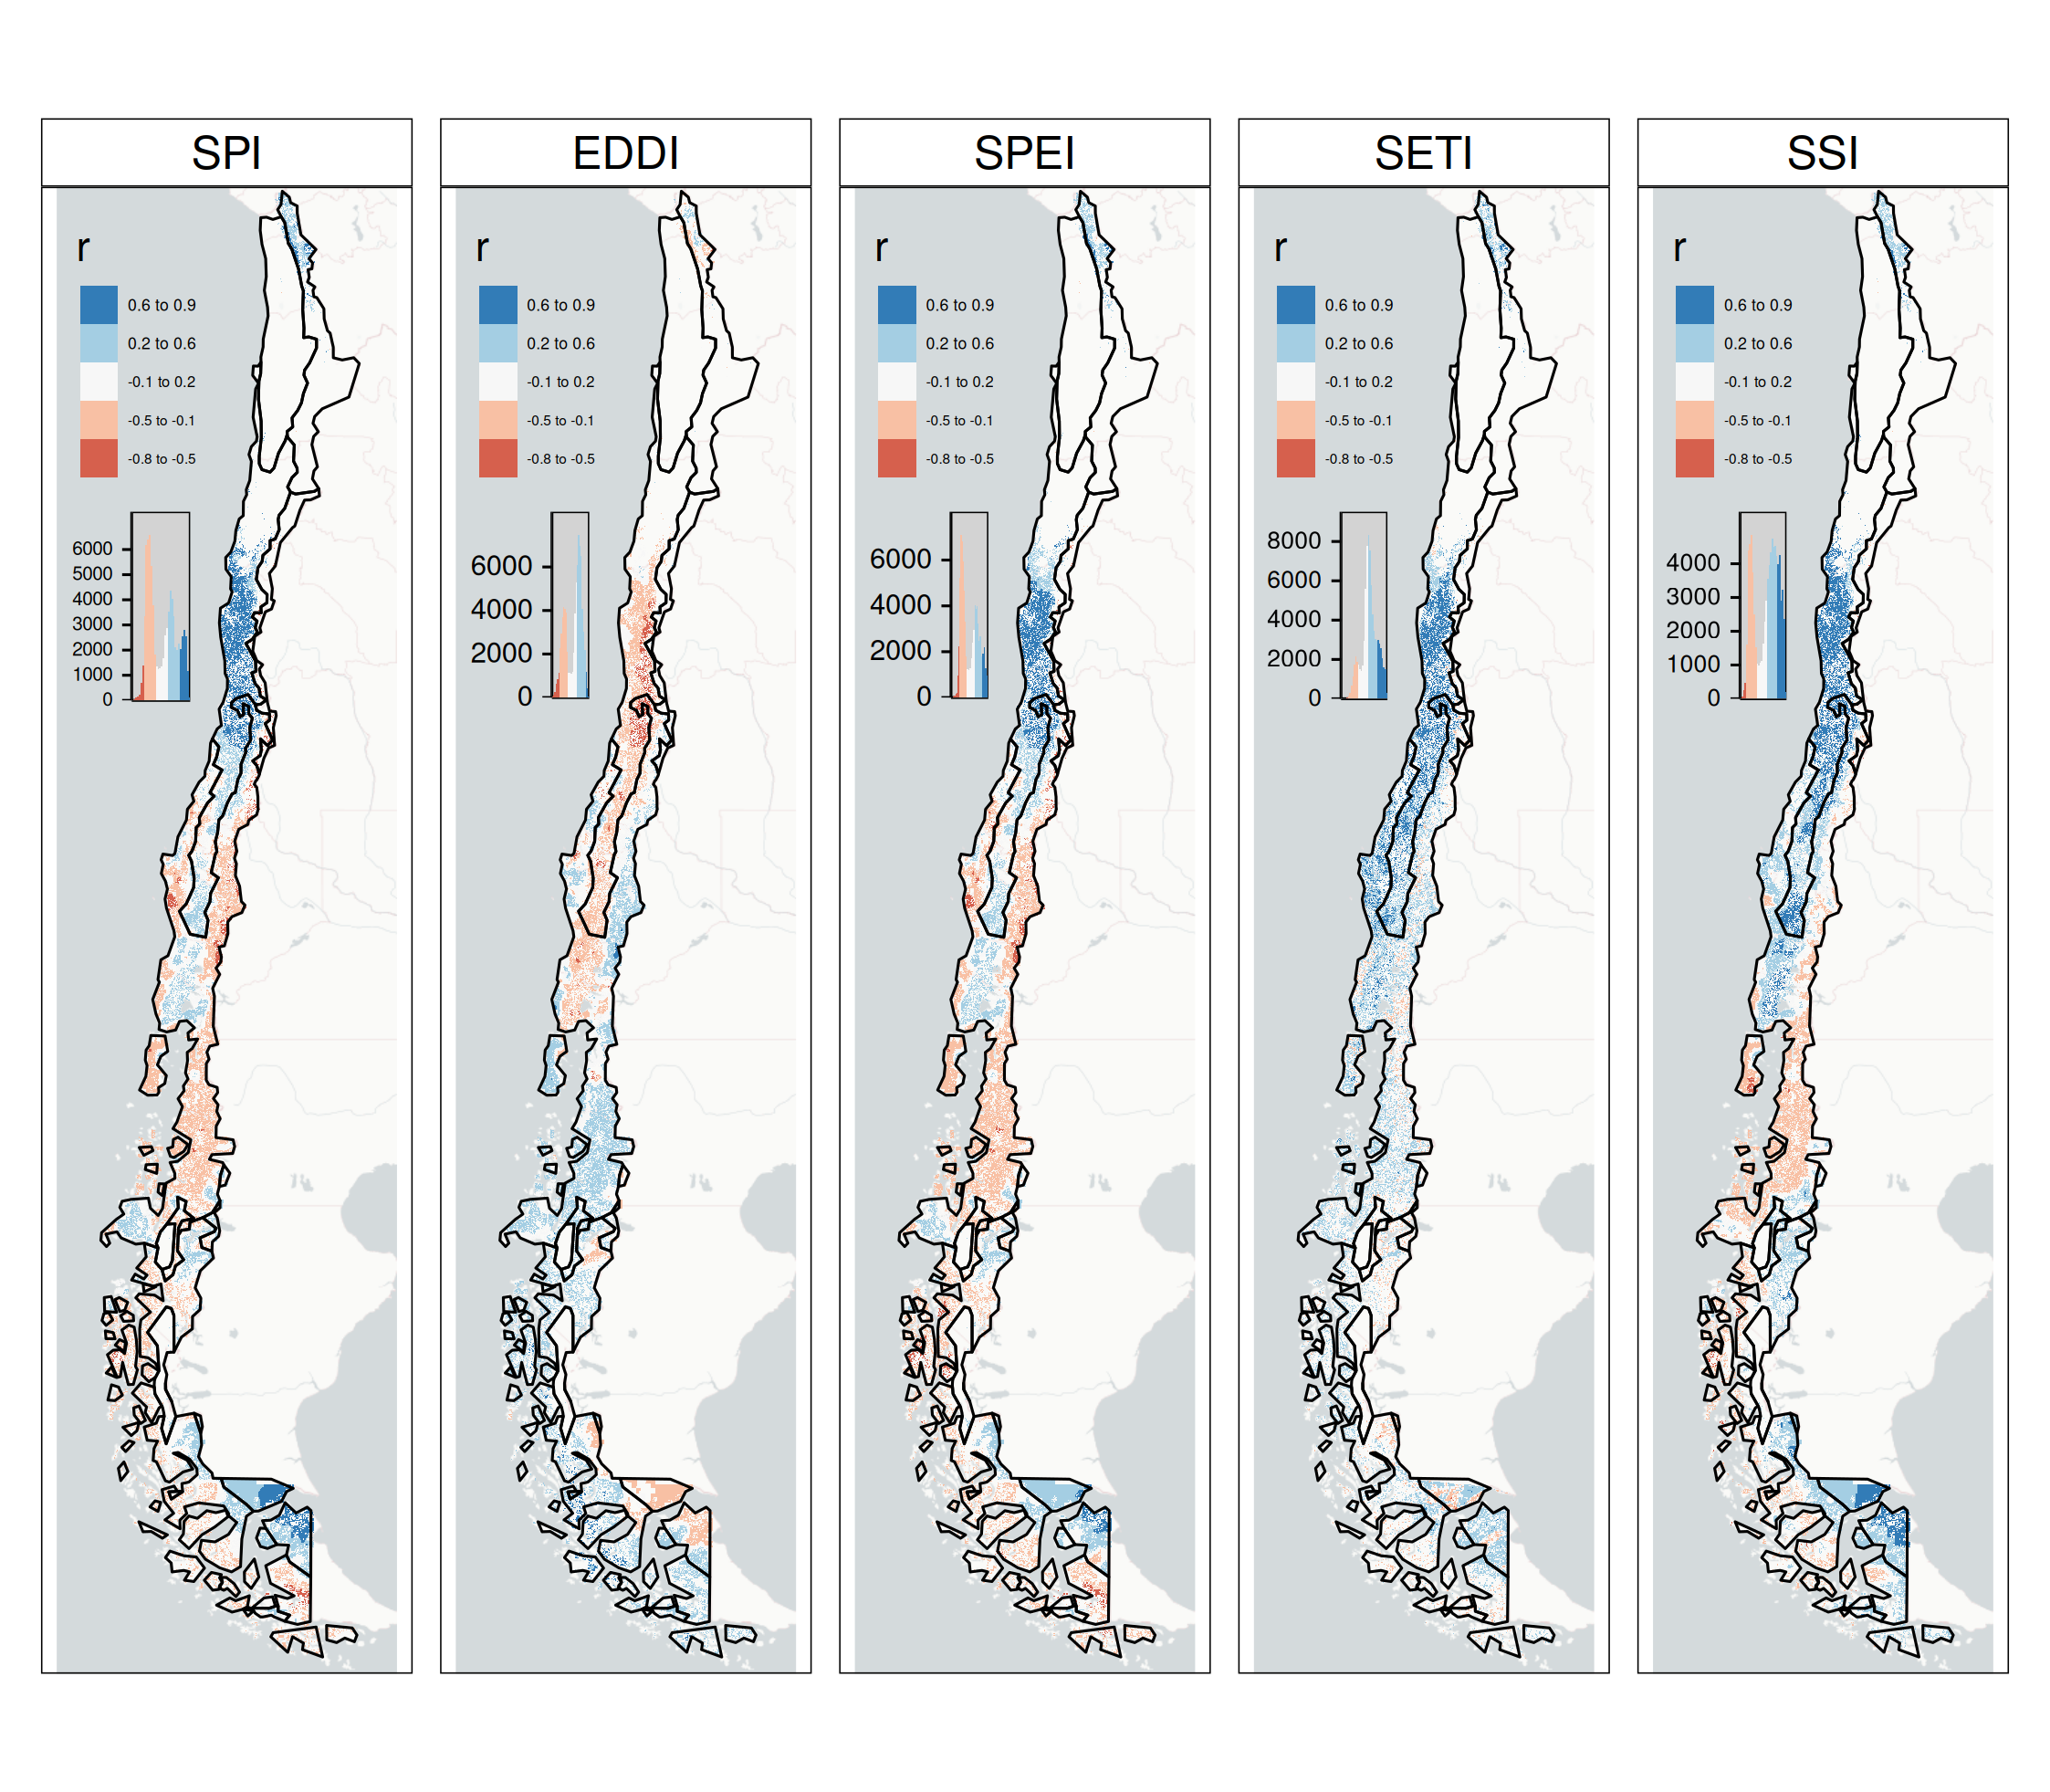
\includegraphics{../output/figs/mapa_cor_r_indices_zcNDVI6.png}

}

\caption{\label{fig-corPerson}Pearson correlation value for the time
scales and drought index that reach the maximum coefficient of
determination. White spaces indicate no significant correlation.}

\end{figure}

Figure~\ref{fig-corTimeScale} shows the time scales that reached the
highest r-squared in the regression analysis between zcNDVI and
different drought indicators over time scales of 1, 3, 6, 12, 24, and 36
months. The spatial variation of time scales reached per index is mostly
for time scales above 12 months. In the case of SSI, the predominant
scales are 6 and 12 months. For all indices, to the north, the time
scales are higher and diminish toward the south until the south part of
``Austral'', where they increase. In Figure~\ref{fig-corPerson}, the map
of Pearson correlation values (r) is shown. The EDDI reached
correlations above 0.5 between ``Norte Chico'' and ``Sur''. The
correlation changes from negative to positive toward the Andes Mountains
and to the sea, just as in the northern part of ``Austral''. The SPI and
SPEI have similar results, with the higher values in ``Norte Chico'' and
``Centro'' being higher than 0.6. Following a similar spatial pattern as
EDDI but with an opposite sign. The SSI showed to be the index that has
a major spatial extension with a higher correlation. It has a similar
correlation to SPI and SPEI for ``Norte Chico'' and ``Centro'', but for
``Sur'' the correlation is higher with SSI.

\begin{table}[!ht]
\caption{Summarry per land cover macroclass and macrozone regarding the correlation between zcNDVI with the drought indices EDDI, SPI, SPEI, and SSI for time scales of 1, 3, 6, 12, 24, and 36. The numbers in each cell indicate the time scale that reached the maximum correlation for the land cover and macrozone, and the color indicates the strength of the r-squared obtained with the index and the time scale. Cells without values indicate that the land cover type was not significant in that macrozone.}
\label{tab-corlandcover}
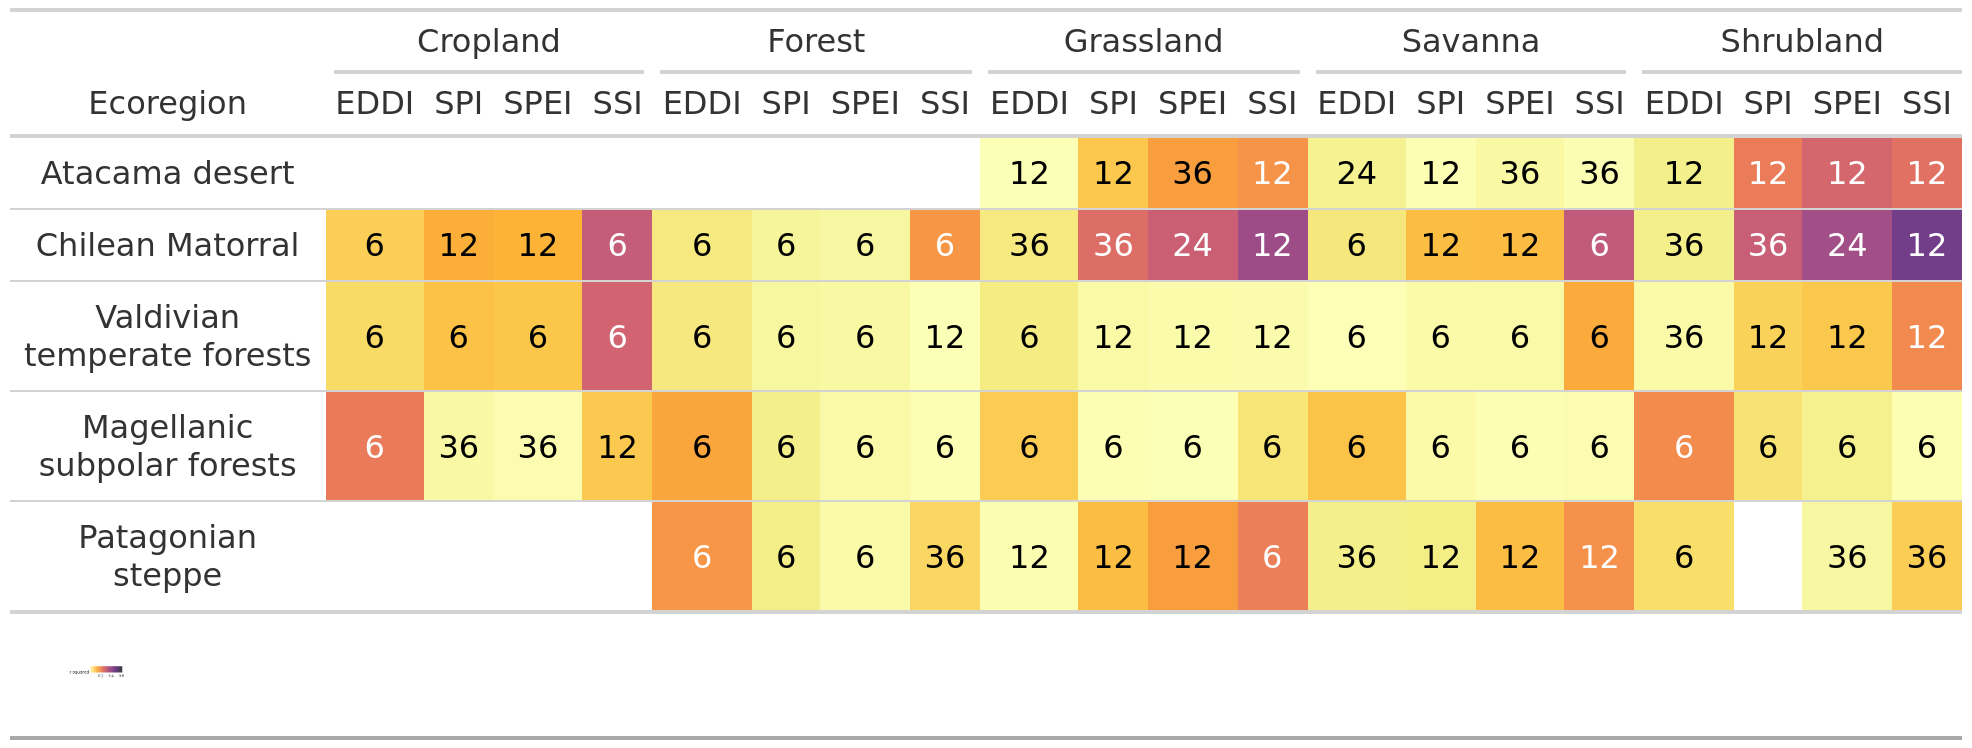
\includegraphics[]{../output/figs/tabla_r_cor_macro_indice.png}
\end{table}

In Table \ref{tab-corlandcover}, we aggregate per macrozone and land
cover the correlation analysis presented in
Figure~\ref{fig-corTimeScale} and Figure~\ref{fig-corPerson}. According
to what is shown, forests is likely to be the most resistant to drought.
Showing that only ``Centro'' is slightly (\(R^2\) = 0.25) impacted by a
12-month soil moisture deficit (SSI-12). In the ``Norte Chico'' and to a
lesser extent in the ``Norte Grande'', it is evident that a SSI-12 with
a \(R^2\) = 0.45 and a decrease in water supply (SPI-36 and SPEI-24 with
\(R^2\) = 0.28 and 0.34, respectively) have an impact on grasslands.
However, this type was unaffected by soil moisture, water supply, or
demand in macrozones further south. The types that show to be most
affected by variation in climate conditions are shrublands, savannas,
and croplands. For savannas in ``Norte Chico'', the SSI-12 and SPI-24
reached an
\(R^2" of 0.74 and 0.58, respectively. This value decreases to the south, but the SSI-12 is still the variable explaining more of the variation in vegetation productivity (\)R\^{}2\$
= 0.45 in ``Centro'' and 0.2 in ``Sur''). In the case of croplands, the
SPEI-12, SPI-36, and SSI-12 explain between 45\% and 66\% of the
variability in ``Norte Chico''. The type of land most impacted by
climatic variation was shrubland, where soil moisture explained 59\% and
precipitation, 37\%, in ``Norte Chico'' and ``Centro'', with SSI-12
being the most relevant variable, then SPI-36 in ``Norte Chico'' and
SPI-24 in ``Sur''.

\hypertarget{discussion}{%
\section{Discussion}\label{discussion}}

\hypertarget{vegetation-water-demand-and-its-relation-to-drought}{%
\subsection{Vegetation water demand and its relation to
drought}\label{vegetation-water-demand-and-its-relation-to-drought}}

In our study, we considered the variation in vegetation productivity in
Chile, specifically in areas without any changes in land cover, to
prevent any misleading conclusions about the increase in water demand
due to land cover change. Our results show a contrasting perspective
regarding the evidence provided by \citet{Vicente-Serrano2022} on a
global scale, who indicates that the increase in drought is led by an
increase in agricultural land, which in turn increases water demand.

Our results indicate that except for the southern part of the country,
the SPI, SPEI, and SSI (water supply) showed declining trends, while the
EDDI (water demand) increased across continental Chile. The trends in
water demand and supply were stronger as the time scales increased,
indicating a long-term reduction in water supply (except for the
southern part) and an increase in water demand by the atmosphere. Also,
we found that there has been a significant declining trend in vegetation
productivity (zcNDVI) since 2000 for the north-central part of the
country, which reached its lowest level between 2020 and 2022 and has
impacted natural and cultivated land. Further, croplands showed a
decrease in surface area for the north-central region, while barren land
increased. We link these changes to a decrease in the water demand from
vegetation because, despite the increase in AED, the surface area for
water-demanding vegetation is declining as well as the biomass
production. However, some questions arise regarding what is occurring
with the cultivated land. Evidence suggests that higher-water-demanding
crops have replaced less demanding crops in the Petorca basin (central
Chile), leading to an increase in water abstraction
\citep{Munoz2020, Duran2020}. Nonetheless, at this scale of analysis,
the effect of higher crop water demand on drought is minor compared to
the decrease in water supply and increase in AED over all land cover
types.

The long-scale trends (e.g., 36 months) demonstrate the impact of
climate change on water availability in Chile, potentially due to an
intense hydrological drought stemming from the ongoing precipitation
deficit and rising AED. But it is likely that in zones most affected by
drought, the main cause is not an increase in vegetation water demand
due to an intensification of cultivated land (e.g., an increase in
irrigated crops) like in other parts of the globe
\citep{Vicente-Serrano2020}. North-central Chile has experienced a
decline in vegetation productivity across land cover types, which is
primarily attributable to variations in water supply and soil moisture.
An increase in water demand, led by an increase in the surface area of
irrigated crops or the change to more water-demanding crops, could
strengthen this trend, however, it escapes the scope of this study.
Future work should focus on the regions where the drought has been more
severe and has a high proportion of irrigated crops to get insight on
the real impact of irrigation on ecosystems in those zones.

\hypertarget{sensitivity-of-land-cover-vegetation-to-short--and-long-term-drought}{%
\subsection{Sensitivity of land cover vegetation to short- and long-term
drought}\label{sensitivity-of-land-cover-vegetation-to-short--and-long-term-drought}}

We analyzed the time series of drought indices and vegetation
productivity per land cover type. Our results indicate that forest is
the type most resistant to drought, and shrublands, savannas, and
croplands have higher sensitivities.

In their study in the Yangtze River Basin in China, \citet{Jiang2020}
analyzed the impact of drought on vegetation using the SPEI and the
Enhanced Vegetation Index (EVI). They found that cropland was more
sensitive to drought than grassland, showing that cropland responds
strongly to short- and medium-term drought (\textless{} SPEI-6). In our
case, the SPEI-12 was the one that most impacted the croplands in
``Norte Chico'' and ``Centro''. In general, most studies show that
croplands are most sensitive to short-term drought (\textless{} SPI-6)
\citep{Zambrano2016, Potopova2015, Dai2020, Rhee2010}. Short-term
precipitation deficits have an impact on soil water, so less water is
available for plant growth. However, we found that in ``Norte Chico'',
an SPI-36 and SPEI-12 had a higher impact, which are associated with
long-term water deficit, and in ``Centro'', an SPI-12 and SPEI-12. Thus,
we hypothesize that this impact could be attributed to the hydrological
drought that has decreased groundwater storage \citep{Taucare2024},
which in turn is impacted by long-term deficits, and consequently, the
vegetation is more dependent on groundwater. In ``Sur'' and ``Austral'',
the correlations between drought indices and vegetation productivity
decrease, as do the time scales that reach the maximum r-squared. The
possible reason for this is that the most resistant types, forest and
grassland, predominate south of ``Centro''. Also, drought episodes have
been less frequent and intense and have had a lower impact on water
availability for vegetation.

In central Chile, \citet{Venegas2022} observed a significant decline in
the overall growth of sclerophyllous moist forests (mediterranean
forests), which they attributed to increased drought conditions.
However, we found that forests are the most resilient land cover class
to drought, with less variation in drought indices. In the ``Sur'',
there is a large domain of planted forests that have replaced native
vegetation since the 1970s
\citep{Heilmayr2016, Heilmayr2020, Miranda2017}, impacting biodiversity
and ecosystem services \citep{Rodriguez2018}. It has recently been shown
that these planted forests are responding positively to climate change,
and it is expected that they will benefit from future climate scenarios
\citep{Carrasco2022}. Further, the forests of the ``Austral'' region
correspond to Patagonian ecosystems, mainly native forests dominated by
tree species of wide niche breadth . Overall, these forests have been
more affected by the increase in temperature than by the reduction in
moisture \citep{Fajardo2023, Holz2018}. These responses have caused
stabilized tree growth, linked to more frequent warm autumns
\citep{Gibson2022}. It has also been observed that these forests have
shown resistance to drought episodes \citep{Fajardo2023}, which might be
attributable to their relatively low growth rate. Supporting this is
\citet{Fathi-Taperasht2022}, who assert that Indian forests are the most
drought-resistant and recover rapidly. Similarly, the work of
\citet{Wu2024}, who analyzed vegetation loss and recovery in response to
meteorological drought in the humid subtropical Pearl River basin in
China, indicates that forests showed higher drought resistance. Using
Vegetation Optical Depth (VOD), kNDVI, and EVI, \citet{Xiao2023} tested
the resistance of ecosystems and found that ecosystems with more forests
are better able to handle severe droughts than croplands. They attribute
the difference to a deeper rooting depth for trees, a higher water
storage capacity, and different water use strategies between forest and
cropland \citep{Xiao2023}.

In another study, \citet{Fuentes2021} evaluated water scarcity and land
cover change in Chile between 29° and 39° south latitude. They used the
one-month SPEI for drought evaluation, which resulted in misleading
results. For instance, they failed to identify a temporal trend in the
SPEI, but they still observed a decline in water availability and a rise
in AED, trends that should have been detectable if they were using
longer SPEI time scales. Thus, according to the results presented in
this study, for the assessment of drought, it is necessary to consider
drought indices on a short- to long-scale basis.

\hypertarget{vegetation-productivity-and-drought}{%
\subsection{Vegetation productivity and
drought}\label{vegetation-productivity-and-drought}}

We found that the 12-month soil moisture deficit affected plant
productivity in all land cover types in Chile. The main external factors
that affect biomass production by vegetation are actual
evapotranspiration and soil moisture, and the rate of ET in turn depends
on the availability of water storage in the root zone. Thus, soil
moisture plays a key role in land carbon uptake and, consequently, in
the production of biomass \citep{Humphrey2021}. The study results showed
that the soil moisture-based drought index (SSI) was better at
explaining vegetation productivity across land cover macroclasses than
meteorological drought indices like SPI, SPEI, and EDDI. According to
\citep{Chatterjee2022} in the early growing season and especially in
irrigated rather than rainfed croplands, soil moisture has better skills
than SPI and SPEI for estimating gross primary production (GPP). Also,
\citet{Zhou2021} indicate that the monthly scaled Standardized Water
Deficit Index (SWDI) can accurately show the effects of agricultural
drought in most of China. \citet{Nicolai2017} also looked at the
time-lag between the SWDI and the Vegetation Condition Index (VCI). They
found that there was little to no time-lag in croplands but a greater
time-lag in forests.

In our case, there is strong spatial variability throughout Chile and
between classes, mainly attributable to climate heterogeneity,
hydrological status, or vegetation resistance to water scarcity. The
semi-arid ``Norte Chico'' and the Mediterranean ``Centro'' were where
SSI had the best performance. In Chile, medium-term deficits of 12
months are more relevant in the response of vegetation for all land
cover types, which decreases to the south, and in the case of croplands,
they seem to react in a shorter time, with six months (SSI-6) in
``Centro''. This variation for croplands could be related to the fact
that in ``Norte Chico'', the majority of crops are irrigated, but to the
south there is a higher proportion of rainfed agriculture, which is most
dependent on the short-term availability of water. Rather, in ``Norte
Chico'', the orchards are more dependent on irrigation, which in turn
depends on the availability of storage water in dams or groundwater
reservoirs, which are affected by long-term drought (e.g., SPI-36).

\hypertarget{drought-information-to-aid-in-adaptation}{%
\subsection{Drought information to aid in
adaptation}\label{drought-information-to-aid-in-adaptation}}

Our findings present valuable information for policymakers in developing
adaptation strategies for droughts. Our results show that the different
climate components, such as AED, water supply, soil moisture, and their
impact on vegetation, should be considered when evaluating the
multi-dimensional nature of drought. Also, for a better understanding of
drought propagation \citep{VanLoon2012} from meteorological to
agricultural and ecological drought, we should consider the climatic
response at different time scales, ranging from short to long.
Additionally, the spatiotemporal characteristics of our results allow us
to distinguish distinct geographical contexts, recognizing the diversity
in climate, but also shedding light on agricultural practices (ranging
from irrigated to dryland farming), technological advancements in
irrigation efficiency, and the region-specific capabilities for drought
adaptation, including groundwater management and reservoir water
storage. This information, combined with agricultural information and
statistics, could provide a strong foundation for the development of
science-based adaptation policies.

In a commitment to fostering informed and dynamic adaptation efforts,
our results are disseminated publicly and continually updated via the
Drought Observatory for Agriculture and Biodiversity of Chile (ODES)
\url{https://odes-chile.org/app/unidades}
\citep{Zambrano2023b, Kunst2023}. This initiative ensures the
availability and easy accessibility of extensive climate data,
facilitating the development of adaptive strategies that are both
responsive to the realities of different regions and grounded in the
latest scientific understanding. The proactive sharing and updating of
such data underscores its key role in enabling policymakers to craft
adaptive measures that are finely tuned to the diverse and evolving
landscapes of drought impacts. Furthermore, the recently promulgated law
about climate change in Chile (Law 21.455,
\url{https://www.bcn.cl/leychile/navegar?idNorma=1177286}), which aims
to implement sectoral adaptation plans for agriculture, forests, and
biodiversity, could benefit from this information.

\hypertarget{conclusion}{%
\section{Conclusion}\label{conclusion}}

We found a significant trend toward decreasing water supply (SPI, SPEI,
and SSI) in most of the Chilean territory, with the exception of the
southern region. The trend is the strongest in the north-central zone.
The whole country showed an increase in water demand (AED) due to
increasing temperatures. The magnitude of the trends is stronger for
longer time scales, which is evidence that there is a prolonged
precipitation shortage and a prolonged increase in AED. The trend in
vegetation productivity in the north-central area is affecting shrubland
and savanna to a greater degree, followed by croplands and forests.

Using Random Forest and variable importance metrics, we assessed how
land cover trends relate to drought indices and found that drought
indices across Chile could explain about 12--41\% of the trends in land
cover types. Drought explains a higher variance in changes in
shrublands, followed by savanna, grasslands, and forest. The changes in
croplands showed the lowest association with drought. We found that the
short- to long-term trend in AED was the most important variable that
could partially explain the observed land cover trend, followed by
long-term trends in precipitation and short-term trends in soil
moisture.

The trends in drought indices are accompanied by multiple land cover
changes in the country, most notably an increase of forest in ``Sur'',
of shrubland and grassland in ``Centro'', and of savanna in ``Centro''
and ``Sur''. In ``Norte Chico'' and ``Centro'', the croplands have been
declining in surface, whereas in ``Sur'', there is an increase in
cultivated land.

The change in vegetation productivity has been severe in the
north-central part of the country for all land cover types, particularly
savanna, shrubland, and croplands. The anomaly in soil moisture over the
past 12 months is the main variable explaining these changes, followed
by anomalies in accumulated precipitation over one to two years. The
variation in AED is likely to exacerbate the drought's impact on
vegetation productivity.

The results of this study provide insightful information that can assist
in developing adaptation measures for Chilean ecosystems to cope with
climate change and drought. This information could be used in the scope
of the national law on climate change, which seeks to implement
adaptation strategies for agriculture, forests, and biodiversity.

\hypertarget{acknowledgment}{%
\section{Acknowledgment}\label{acknowledgment}}

The National Research and Development Agency of Chile (ANID) funded this
study through the drought emergency project FSEQ210022, Fondecyt
Iniciación N°11190360, Fondecyt Postdoctorado N°3230678, and Fondecyt
Regular N°1210526. The companies Garces Fruit and CER Analytics provided
access to the \emph{in-situ} soil moisture data used in this work.


\renewcommand\refname{References}
  \bibliography{references.bib}


\end{document}
